% !TEX program = tectonic
% Rapport « Congress Trading Signal · couche données » — récit chronologique.
% Tous les chiffres sont recalculés depuis les tables FINAL
% (data/house/tables/{an}/06_house_{an}_FINAL.csv, data/senate/tables/{an}/06_senate_{an}_FINAL.csv)
% et la source de vérité chiffrée tests/regression/audit_metrics.py + common/quality.py.
\documentclass[11pt,a4paper]{article}
\usepackage[T1]{fontenc}
\usepackage{lmodern}
\usepackage[utf8]{inputenc}
\usepackage[french]{babel}
\usepackage[a4paper,margin=2cm]{geometry}
\usepackage{booktabs}
\usepackage{longtable}
\usepackage{array}
\usepackage{enumitem}
\usepackage{xcolor}
\usepackage{titlesec}
\usepackage{graphicx}
\usepackage{needspace}
\usepackage{hyperref}
\usepackage{underscore}
\usepackage{amssymb}
\usepackage{textcomp}
\usepackage{newunicodechar}
\usepackage{tikz}
\usetikzlibrary{shapes.geometric,arrows.meta,positioning,fit,backgrounds,calc}

% Caractères Unicode → commandes LaTeX (fontes T1 sans ces glyphes)
\newunicodechar{→}{\ensuremath{\rightarrow}}
\newunicodechar{—}{\textemdash}
\newunicodechar{–}{\textendash}
\newunicodechar{…}{\ldots}
\newunicodechar{−}{\ensuremath{-}}
\newunicodechar{·}{\textperiodcentered}
\newunicodechar{œ}{\oe}
\newunicodechar{Œ}{\OE}
\newunicodechar{≈}{\ensuremath{\approx}}
\newunicodechar{×}{\ensuremath{\times}}
\newunicodechar{≤}{\ensuremath{\leq}}
\newunicodechar{≥}{\ensuremath{\geq}}
\newunicodechar{↔}{\ensuremath{\leftrightarrow}}
\newunicodechar{★}{\ensuremath{\star}}
% Guillemets : mapper les « » littéraux vers \og/\fg de babel — rendu ET extraction corrects.
\newunicodechar{«}{\og}
\newunicodechar{»}{\fg{}}

\hypersetup{colorlinks=true,linkcolor=blue!55!black,urlcolor=blue!55!black,
  pdftitle={Congress Trading Signal — Couche données}, pdfauthor={Alice Lemaire}}

\definecolor{coreC}{RGB}{37,99,159}
\definecolor{houseC}{RGB}{30,110,90}
\definecolor{senateC}{RGB}{120,60,150}
\definecolor{dataC}{RGB}{176,110,14}
\definecolor{testC}{RGB}{150,40,40}
\definecolor{netC}{RGB}{190,55,55}
\definecolor{offC}{RGB}{40,120,60}

\newcommand{\co}[1]{\texttt{\small #1}}
\newcommand{\netflag}{\textcolor{netC}{\small$\bullet$ réseau/API}}
\newcommand{\offflag}{\textcolor{offC}{\small$\bullet$ offline}}
% Encart « dans la source » sobre (filet à gauche, sans boîte colorée)
\newcommand{\srcex}[1]{\par\smallskip\noindent{\color{coreC}\rule{2pt}{\baselineskip}}\hspace{6pt}\begin{minipage}{\dimexpr\linewidth-16pt}\small\textit{Dans la source.}\ #1\end{minipage}\par\smallskip}
% Encart « hypothèse révisée » (filet ocre) — la valeur recherche des choix corrigés, fondue dans le récit.
\newcommand{\rev}[1]{\par\smallskip\noindent{\color{dataC}\rule{2pt}{\baselineskip}}\hspace{6pt}\begin{minipage}{\dimexpr\linewidth-16pt}\small\textit{\color{dataC}Hypothèse explorée puis révisée.}\ #1\end{minipage}\par\smallskip}

\titleformat{\section}{\Large\bfseries\color{coreC}}{\thesection}{0.6em}{}
\titleformat{\subsection}{\large\bfseries}{\thesubsection}{0.6em}{}
\titlespacing{\section}{0pt}{1.3em}{0.4em}
\titlespacing{\subsection}{0pt}{0.8em}{0.25em}

\tikzset{
  step/.style={rectangle, rounded corners=2pt, draw=#1, line width=0.8pt, fill=#1!8,
               text width=3.4cm, align=center, minimum height=0.95cm, font=\small},
  file/.style={rectangle, draw=gray!55, fill=gray!7, text width=3.4cm, align=center,
               font=\scriptsize\ttfamily, minimum height=0.55cm},
  lyr/.style={rectangle, rounded corners=3pt, draw=#1, line width=1pt, fill=#1!8,
              align=center, font=\small, minimum height=1.1cm},
  arr/.style={-{Latex[length=2.4mm]}, line width=0.9pt, draw=gray!65},
}

\setlength{\parindent}{0pt}
\setlength{\parskip}{4pt}
\setlength{\emergencystretch}{3em}
\renewcommand{\arraystretch}{1.2}

\begin{document}

% ============================ EN-TÊTE COMPACT ============================
\begin{center}
{\small\itshape Document de recherche — livrable Ramify}\\[3pt]
{\Huge\bfseries\color{coreC} Congress Trading Signal}\\[3pt]
{\Large\bfseries La couche données}\\[5pt]
{\normalsize Extraction, identification, enrichissement et validation honnête des déclarations\\
boursières du Congrès américain — Chambre \emph{et} Sénat, 2020--2026}\\[6pt]
{\large\bfseries Alice Lemaire}\quad\textperiodcentered\quad{\small\today}
\end{center}
\vspace{2pt}\hrule\vspace{6pt}

% ============================ RÉSUMÉ ============================
\section*{Résumé}
Les membres du Congrès américain déclarent leurs transactions boursières sous le \emph{STOCK Act}~; ces
déclarations, exploitées par une stratégie de \emph{copy-trading}, exigent au préalable une couche
données propre, traçable et honnêtement validée. Ce rapport raconte la construction de cette couche,
étape par étape — de l'acquisition des sources jusqu'à la table finale enrichie et validée. Le pipeline
reconstruit \textbf{90\,487 transactions} sur deux chambres et sept ans (2020--2026)~: \textbf{81\,646}
pour la Chambre (32\,676 électronique + 48\,970 OCR) et \textbf{8\,841} pour le Sénat (7\,161
électronique + 1\,680 papier OCR). Chaque transaction est rattachée à son auteur (\textbf{99,99\,\%} des
lignes Chambre, \textbf{100\,\%} au Sénat), enrichie (ticker, secteur \textbf{GICS$\rightarrow$ETF SPDR},
type d'actif, montant \emph{midpoint}, ancienneté), aboutissant à la \textbf{table 12/12 champs}. La
validation externe contre Quiver — \textbf{jamais réinjecté} — est conduite par \textbf{scope}
(électronique / OCR / les deux)~: au niveau transaction, on retrouve \textbf{98,2\,\%} des trades Quiver
sur l'électronique de la Chambre, \textbf{68,3\,\%} sur l'OCR et \textbf{86,2\,\%} sur l'ensemble~;
\textbf{99,4\,\%} au Sénat. Cette validation par scope corrige une idée reçue~: \textbf{Quiver voit bien
le papier de la Chambre} (les gros déposants-papier comme Khanna y figurent) — l'OCR Chambre est donc
\emph{validé en externe}, et la seule vraie limite est la \textbf{lecture OCR des dates manuscrites}. La
correction est figée par un \textbf{golden octet-à-octet} (\textbf{125} fichiers Chambre, \textbf{76}
Sénat) et des reproductions fonction-par-fonction. Chaque étape est exposée selon le même fil~: le
\textbf{problème} concret, la \textbf{façon dont il est résolu} (avec la fonction réelle), et le
\textbf{résultat chiffré}.

% ============================ 1. INTRODUCTION ============================
\section{Introduction \& contexte}
Depuis le \textbf{STOCK Act} (2012), les membres du Congrès américain doivent divulguer publiquement
leurs transactions sur titres dans un \emph{Periodic Transaction Report} (PTR), en principe sous
\textbf{45 jours}. L'intuition de recherche — documentée académiquement (Ziobrowski \emph{et al.}
2004/2011, Karadas 2019) — est que ces personnes, par leur appartenance à des commissions clés
(Finance, \emph{Armed Services}, Intelligence) ou leur exposition à l'information, produisent par leurs
déclarations un \textbf{signal potentiellement exploitable}. Une stratégie de \emph{copy-trading}
consiste à répliquer ces transactions \emph{après} leur publication (anti-\emph{look-ahead}~: on date
chaque transaction par sa date de divulgation, jamais par une date postérieure connue).

Avant toute stratégie, il faut une \textbf{couche données} irréprochable~: extraire fidèlement les
déclarations des deux chambres, les rattacher à la bonne personne, les enrichir (ticker, secteur,
montant) et les valider honnêtement. C'est l'objet de ce rapport. La stratégie et le backtest associés
constituent un travail de recherche séparé, hors du périmètre traité ici.

% ============================ 2. SOURCES ============================
\section{Sources \& acquisition}
\label{sec:sources}

\subsection{Les trois dates — et le principe anti-\emph{look-ahead}}
Une déclaration porte \textbf{deux dates} (parfois trois), qu'il ne faut pas confondre~:
\begin{itemize}[nosep,leftmargin=1.4em]
\item \co{transaction_date} — \textbf{quand le trade a eu lieu}, lue \emph{dans} le PTR (la ligne de
transaction elle-même). C'est la date « économique ».
\item \co{disclosure_date} — \textbf{quand la déclaration a été déposée}. Côté Chambre, c'est le
\co{FilingDate} de l'index XML (\co{house/digital.py}, l.\,262)~; côté Sénat, la dernière date de la
liste eFD (\co{senate/digital.py}, l.\,100). C'est la date « publique »~: avant elle, l'information
n'existe pas pour un copieur.
\item \co{notification_date} — \textbf{Chambre OCR seulement}~: certains formulaires papier portent une
date de notification distincte, conservée quand elle est lisible.
\end{itemize}
\textbf{Pourquoi cette distinction est structurante.} Une stratégie ne peut copier qu'\emph{après}
publication~: on fenêtre et on date donc tout par la \co{disclosure_date}, jamais par la
\co{transaction_date} (qui, elle, est antérieure et inconnue du marché au moment du dépôt). La clé
naturelle d'une transaction (§\ref{sec:table}) \textbf{exclut volontairement} la \co{disclosure_date}~:
deux dépôts du même trade (un dépôt initial puis un amendement) doivent rester \emph{une} transaction,
pas deux. La divulgation sert d'axe temporel et d'anti-\emph{look-ahead}, pas d'identité.

\subsection{Où et comment on récupère les déclarations}
\textbf{Chambre — \emph{House Clerk}.} Source publique, sans barrière. Pour chaque année, le Clerk publie
une archive ZIP contenant un \textbf{index XML} (\co{\{an\}FD.xml}) qui liste tous les dépôts~: \co{DocID},
nom (\co{Last}/\co{First}), \co{StateDst}, \co{FilingType} et \co{FilingDate}. On lit cet index
(\co{house/digital.py:load_ptr_index}), on filtre \co{FilingType=P} (les PTR), et on déduit l'URL du PDF
de chaque dépôt (\co{resolve_pdf_path}). \textbf{C'est en ouvrant le PDF qu'on décide} s'il est lisible
ou scanné (\co{build_manifest}, §\ref{sec:tri}).

\textbf{Sénat — eFD (\emph{Electronic Financial Disclosure}).} Plus fermé~: un \textbf{garde-fou CSRF}.
Il faut d'abord accepter un formulaire d'accord (\co{senate/digital.py:accept_agreement}~: GET pour un
\co{csrftoken}, puis POST \co{prohibition_agreement} avec \co{csrfmiddlewaretoken} et l'en-tête
\co{X-CSRFToken}). On interroge ensuite l'API de recherche (\co{fetch_ptr_list},
\co{report_types=[11]} = PTR)~; chaque dépôt y porte un \co{kind} — \co{ptr} (déclaration HTML
électronique) ou \co{paper} (image \co{.gif} scannée). \co{fetch_report} récupère chaque déclaration. On
reste « poli » (pause entre requêtes, aucun contournement) et on \textbf{cache tout sur disque} — un
re-run ne re-télécharge rien.

\subsection{D'où viennent les informations sur les élus (le référentiel)}
\label{sec:reference}
Une déclaration ne donne qu'un \emph{nom}. Pour savoir que « Buddy Carter » siège à la \emph{Chambre},
qu'il est Républicain et dans telle commission, il faut un \textbf{référentiel des élus}. On utilise le
jeu de données ouvert et maintenu \textbf{\emph{congress-legislators}}
(\co{unitedstates.github.io}), avec un \textbf{repli sur des YAML embarqués} dans le dépôt
(\co{data/\{chambre\}/reference/legislators-*.yaml} + \co{committees-*.yaml}) — ainsi le pipeline reste
reproductible hors-ligne. \co{common/reference.py:load_reference} en tire, pour chaque \co{bioguide_id}~:
la \textbf{chambre} (déduite du dernier mandat, \co{term.type}), le \textbf{parti}, et les
\textbf{commissions} (\co{bio_to_committees}), avec un drapeau « commission clé » propre à chaque chambre.
Ce référentiel est \emph{partagé} par les deux chambres~; seul le \textbf{matcher} nom$\rightarrow$bioguide
est spécifique (\co{house/identity.py}, \co{senate/identity.py}, §\ref{sec:identity}).

\subsection{Pourquoi l'API Claude Vision pour les scans}
\label{sec:vision}
La moitié des déclarations de la Chambre, et tout le papier du Sénat, n'existent que comme
\textbf{images} (PDF scannés, \co{.gif}) — souvent \emph{couchées}, parfois \emph{manuscrites}, avec des
montants en \textbf{cases à cocher}. Un OCR classique (Tesseract) bute sur ces formulaires~: il rend du
texte brut sans structure, et lit très mal une page tournée ou une écriture à la main. On utilise donc
l'\textbf{API Claude Vision} (modèle \co{claude-sonnet-4-6}), qui fait d'une pierre deux coups~: elle
\emph{lit} l'image \emph{et} la \emph{structure} directement en transactions. Concrètement
(\co{common/vision_ocr.py}, \co{house/ocr.py}, \co{senate/ocr_engine.py})~: l'appel force un
\co{tool_use} sur l'outil \co{record_transactions} (le modèle \emph{doit} répondre dans un schéma JSON
strict — pas de texte libre à re-parser), avec \textbf{7 tentatives} et \emph{backoff}, et un
\textbf{cache versionné par \co{prompt_sha}} (un re-run ne re-paie que les lots en erreur~: 0 appel si
rien n'a changé). Le choix du modèle est assumé~: \co{claude-sonnet-4-6} suffit ici (une sonde Opus n'a
pas amélioré le point dur — les dates manuscrites — pour un coût $\approx\!\times 3$, §\ref{sec:hocr}).

\subsection{Quiver = vérification externe \emph{uniquement}}
Quiver Quantitative (agrégateur commercial) sert de \textbf{vérité-terrain indépendante}. Il n'est
\emph{jamais} réinjecté dans nos tables~: on mesure si notre extraction concorde, on ne la complète pas.
C'est une règle structurante du projet (validation détaillée en §\ref{sec:quiver}).

% ============================ 3. ARCHITECTURE ============================
\section{Architecture \& méthodologie}
\label{sec:archi}

\subsection{Un contrat partagé + deux orchestrateurs jumeaux + données + tests}
\label{sec:archi-couches}
Le code est organisé en un \textbf{contrat universel partagé} (\co{common/}, 9 modules) que
\textbf{deux orchestrateurs symétriques} (\co{house/} et \co{senate/}) utilisent. \co{common/} ne contient
que ce qui est \emph{vraiment} commun aux deux chambres (ou au pipeline, à la qualité, à l'ancienneté)~;
tout ce qui \emph{diffère} par chambre — le matcher d'identité, les montants, le ticker, l'OCR de
production, la validation Quiver — vit dans \co{house/} et \co{senate/}, qui sont des \textbf{jumeaux}.
Les données et les tests complètent l'ensemble.

\begin{center}
\begin{tikzpicture}
\node[lyr=houseC, text width=5.4cm] (h) at (-3.2,1.4) {\textbf{\color{houseC}house/} \;(7 modules)\\[1pt]\footnotesize orchestrateur Chambre\\\footnotesize \co{digital}·\co{ocr}·\co{identity}·\co{amounts}\\\footnotesize \co{tickers}·\co{quiver}·\co{echantillon}};
\node[lyr=senateC, text width=5.4cm] (s) at (3.2,1.4) {\textbf{\color{senateC}senate/} \;(8 modules)\\[1pt]\footnotesize orchestrateur Sénat\\\footnotesize \co{digital}·\co{ocr}·\co{ocr_engine}·\co{fusion}\\\footnotesize \co{identity}·\co{ticker}·\co{quiver}·\co{census_probe}};
\node[lyr=coreC, text width=11.4cm] (c) at (0,-0.5) {\textbf{\color{coreC}common/} \;(9 modules) — le contrat UNIVERSEL partagé\\[1pt]\footnotesize reference · schema · sector\_enrich · vision\_ocr · crosscheck · quality · enrich\_tenure · \textbf{pipeline} · quiver\_scopes};
\node[lyr=dataC, text width=7.6cm] (d) at (-2.0,-2.3) {\textbf{\color{dataC}data/} — entrées \& sorties\\\footnotesize \co{\{chambre\}/tables/\{an\}/}, PDF, scans, caches, référentiels};
\node[lyr=testC, text width=3.0cm] (t) at (3.7,-2.3) {\textbf{\color{testC}tests/}\\\footnotesize filet « zéro changement »};
\draw[arr] (h) -- (c); \draw[arr] (s) -- (c);
\draw[arr] (c) -- (d); \draw[arr] (c.south) -- (t.north);
\end{tikzpicture}
\end{center}
La symétrie est volontaire~: \co{house/} et \co{senate/} portent les \emph{mêmes} rôles
(\co{digital}/\co{ocr}/\co{identity}/\co{quiver}\dots), seules leurs implémentations diffèrent là où les
sources diffèrent. La seule asymétrie de structure est \co{senate/fusion.py} (expliquée en
§\ref{sec:socr})~; côté Chambre, la fusion vit dans \co{house/ocr.py}.

\subsection{Le pipeline : le schéma à lire en premier}
\label{sec:pipeline}
\co{common/pipeline.py} (fonction \co{build_steps}) enchaîne \textbf{6 étapes} en sous-processus~; un
\textbf{7\textsuperscript{e}} traitement — le rapport qualité (\co{common/quality.py}) — se lance
séparément, hors-ligne et en lecture seule. Le schéma ci-dessous montre, en plus des 6 étapes, l'\textbf{étape
0 d'acquisition \& de tri} (\S\ref{sec:sources}) et la \textbf{fourche électronique/OCR} qui structure
tout le reste.

\begin{center}
\begin{tikzpicture}[node distance=5mm]
% Étape 0 — acquisition & tri
\node[step=dataC, fill=dataC!12, text width=6.6cm] (acqH) at (-4.1,0)
  {\textbf{0a. Chambre — acquisition} \netflag\\[1pt]\footnotesize ZIP Clerk → index XML \co{\{an\}FD.xml} → \co{FilingType=P} → PDF → \textbf{tri} \co{bool(text)} → \co{04_manifest}};
\node[step=dataC, fill=dataC!12, text width=6.6cm] (acqS) at (4.1,0)
  {\textbf{0b. Sénat — acquisition} \netflag\\[1pt]\footnotesize eFD → accord CSRF → \co{report_types=[11]} → liste avec \co{kind} (\co{ptr} / \co{paper})};
% Orchestrateur
\node[step=coreC, fill=coreC!15, text width=11cm, below=7mm of $(acqH)!0.5!(acqS)$] (orch)
  {\textbf{python -m common.pipeline}\\[1pt]\footnotesize \co{build_steps()} : 6 étapes en sous-processus, puis le rapport qualité (offline)};
% Colonne Chambre
\node[step=houseC, below=8mm of orch, xshift=-3.9cm] (hd) {\textbf{1.} \co{house.digital}\\\footnotesize PTR lisibles → parsing \netflag};
\node[file, below=4mm of hd] (hdf) {06\_house\_\{an\}\_transactions.csv};
\node[step=houseC, below=4mm of hdf] (ho) {\textbf{2.} \co{house.ocr}\\\footnotesize scans → Vision · fusion · ticker · secteur · Quiver \netflag};
\node[file, below=4mm of ho, fill=houseC!12] (hof) {06\_house\_\{an\}\_FINAL.csv};
% Colonne Sénat
\node[step=senateC, below=8mm of orch, xshift=3.9cm] (sd) {\textbf{3.} \co{senate.digital}\\\footnotesize eFD HTML → parsing \netflag};
\node[file, below=4mm of sd] (sdf) {06\_senate\_\{an\}\_transactions.csv};
\node[step=senateC, below=4mm of sdf] (so) {\textbf{4.} \co{senate.ocr}\\\footnotesize papier \co{.gif} → Vision \netflag};
\node[file, below=4mm of so] (sof) {06b\_senate\_\{an\}\_ocr.csv};
\node[step=senateC, below=4mm of sof] (sf) {\textbf{5.} \co{senate.fusion}\\\footnotesize fusion + ticker + secteur + Quiver};
\node[file, below=4mm of sf, fill=senateC!12] (sff) {06\_senate\_\{an\}\_FINAL.csv};
% Convergence
\node[step=offC, below=9mm of sff, xshift=-3.9cm, text width=7.8cm] (et)
  {\textbf{6.} \co{common.enrich_tenure} \offflag\\\footnotesize ajoute \co{years_in_office} aux 14 tables FINAL};
\node[step=offC, below=5mm of et, text width=7.8cm] (q)
  {\textbf{7.} \co{common.quality} \offflag\\\footnotesize 6 contrôles → \co{RAPPORT_QUALITE.md} + figures};
\draw[arr] (acqH) -- (orch); \draw[arr] (acqS) -- (orch);
\draw[arr] (orch) -| (hd);
\draw[arr] (orch) -| (sd);
\draw[arr] (hd)--(hdf); \draw[arr] (hdf)--(ho); \draw[arr] (ho)--(hof);
\draw[arr] (sd)--(sdf); \draw[arr] (sdf)--(so); \draw[arr] (so)--(sof); \draw[arr] (sof)--(sf); \draw[arr] (sf)--(sff);
\draw[arr] (hof) |- (et); \draw[arr] (sff) -- (et);
\draw[arr] (et)--(q);
\end{tikzpicture}
\end{center}

\subsection{La numérotation des fichiers : des étiquettes de rôle, pas l'ordre d'exécution}
\label{sec:numbering}
Sur le disque, le \textbf{préfixe} d'un fichier indique le \textbf{rôle} (la famille d'étape) de la table.
C'est ce qui rend la couche données lisible sans documentation externe. \textbf{Attention}~: le préfixe
n'est \emph{pas} strictement l'ordre d'exécution. Plusieurs tables d'un même numéro sont écrites par des
modules différents, et certains numéros élevés sont produits \emph{avant} des numéros plus petits — par
exemple, au Sénat, \co{07_quiver_comparison} (validation de la piste électronique) est écrit dès l'étape
\co{senate.digital}, donc \emph{avant} l'OCR \co{06b} et la fusion \co{06\_…\_FINAL}. L'ordre réel est
celui du pipeline (§\ref{sec:pipeline})~; les préfixes en sont une \emph{approximation lisible}.

\begin{center}\small
\begin{tabular}{>{\ttfamily}p{2.5cm} p{9.6cm} >{\ttfamily\footnotesize}p{3.4cm}}
\toprule
\normalfont\bfseries Préfixe & \bfseries Rôle & \normalfont\bfseries Écrit par \\
\midrule
03\_ & index des PTR (\co{FilingType=P}) dans la fenêtre \emph{(Chambre)} & house.digital \\
04\_ & manifeste de tri~: lisible / non\_lisible / absent \emph{(Chambre)} & house.digital \\
05\_ & échecs de parsing & *.digital \\
06\_ & table \textbf{électronique} (PTR lisibles / eFD HTML) & *.digital \\
06b\_ & table \textbf{OCR} (scans Chambre / papier Sénat) & house.ocr / senate.fusion \\
06c\_ & échecs OCR & house.ocr / senate.ocr \\
06d\_ & comparaison OCR↔Quiver \emph{(Chambre)} & house.ocr \\
06\_…\_FINAL & \textbf{électronique + OCR fusionnés}, enrichis & house.ocr / senate.fusion \\
07\_ & comparaison Quiver de la piste électronique (par déposant) & *.digital / fusion \\
07b\_ & trades Quiver manquants, piste électronique \emph{(Chambre)} & house.digital \\
07c--07f\_ & \textbf{réconciliation Quiver 3 scopes} (txn / champs / ticker / only-Quiver) & house.ocr / senate.fusion \\
07g\_ & décomposition Quiver par \textbf{type d'actif} & house.ocr / senate.fusion \\
07h\_ & décomposition Quiver par \textbf{cluster de scan} \emph{(Chambre)} & house.ocr \\
08\_ & cross-check « semaine 1 » \emph{(Chambre)} & house.digital \\
00\_ & tableaux de bord (statut par an / final) \emph{(Sénat)} & senate.digital / fusion \\
\_préfixe & caches \& brouillons (\co{_quiver_*_cache}, \co{_scan_census_547}…) & divers \\
\bottomrule
\end{tabular}
\end{center}
\textbf{Pourquoi cette asymétrie~?} La Chambre doit \emph{calculer} elle-même le tri lisible/scanné (d'où
\co{03}/\co{04}~: ouvrir chaque PDF, tester sa couche texte), tandis que le Sénat reçoit le \co{kind}
\emph{déjà donné} par l'API eFD (pas de manifeste à produire). Les décompositions par cluster (\co{07h})
n'existent qu'à la Chambre, seule à disposer d'un census de scans (§\ref{sec:hocr}). Les
réconciliations \co{07c--07g} sont, elles, \textbf{symétriques}~: les deux chambres les produisent.

% ============================ 4. CONSTRUCTION (RÉCIT) ============================
\section{Construction de la donnée, étape par étape}
\label{sec:construction}

Cette section suit une transaction \emph{dans l'ordre où le pipeline la construit} — de l'acquisition
jusqu'à la ligne enrichie, validée, de la table finale. Le \textbf{schéma maître} ci-dessous en est le
résumé visuel complet~: il montre les \textbf{cinq formes} sous lesquelles une déclaration arrive
(deux chambres, et selon le type de document), comment chacune est extraite, puis le tronc \emph{commun}
— identité, enrichissement, table finale, validation. Le récit qui suit déroule chaque étape~: le
\textbf{problème} concret, \textbf{comment on le résout} (avec la fonction réelle), le \textbf{résultat}
chiffré. Les choix \emph{révisés} en cours de route sont signalés par un encart ocre.

\begin{center}
\begin{tikzpicture}[every node/.style={font=\footnotesize}, node distance=4mm]
% --- Acquisition (2 boîtes) ---
\node[step=dataC, fill=dataC!10, text width=5.0cm] (acqH) at (-4.0,0)
  {\textbf{\color{houseC}Chambre} — ZIP Clerk → index XML → \co{FilingType=P} → PDF};
\node[step=dataC, fill=dataC!10, text width=5.0cm] (acqS) at (4.0,0)
  {\textbf{\color{senateC}Sénat} — eFD (CSRF) → \co{report_types=[11]} → liste \co{kind}};
% --- Tri / type de document : 4 feuilles + C exclu ---
\node[step=houseC, text width=3.0cm] (hpdf) at (-6.0,-2.0) {\textbf{PDF lisible}\\\footnotesize couche texte};
\node[step=houseC, text width=3.0cm] (hscan) at (-2.6,-2.0) {\textbf{scan tapé} A/B\\\footnotesize image (couchée)};
\node[step=senateC, text width=3.0cm] (shtml) at (2.6,-2.0) {\textbf{HTML eFD}\\\footnotesize page web};
\node[step=senateC, text width=3.0cm] (sgif) at (6.0,-2.0) {\textbf{papier} \co{.gif}\\\footnotesize image droite};
\node[file, text width=2.6cm, fill=gray!12, draw=testC] (hC) at (-2.6,-3.4) {scan manuscrit C → exclu par défaut};
% --- Extraction ---
\node[step=houseC, text width=3.0cm] (hpar) at (-6.0,-4.4) {\co{parse_ptr}\\\footnotesize \co{TXN_RE}, déterministe};
\node[step=houseC, text width=3.0cm] (hvis) at (-2.6,-5.0) {OCR \textbf{Vision}\\\footnotesize deskew 4 rotations};
\node[step=senateC, text width=3.0cm] (spar) at (2.6,-4.4) {\co{pd.read_html}\\\footnotesize \co{_find_col} flou};
\node[step=senateC, text width=3.0cm] (svis) at (6.0,-4.4) {OCR \textbf{Vision}\\\footnotesize sans deskew};
% --- Convergence ---
\node[step=coreC, fill=coreC!12, text width=12.4cm] (conv) at (0,-6.6)
  {\textbf{lignes normalisées} — déclarant, \co{transaction_date}, \co{disclosure_date}, \co{asset_description}, \co{operation_type}, \co{amount_range}, \co{owner}};
% --- Tronc commun ---
\node[step=coreC, text width=12.4cm] (ident) at (0,-8.0)
  {\textbf{identité} — \co{house/senate.identity} sur le référentiel partagé (\co{common.reference}) → \co{bioguide_id}, \co{party}, \co{committee_membership}};
\node[step=coreC, text width=12.4cm] (enr) at (0,-9.4)
  {\textbf{enrichissement} — ticker (\co{tickers}/LLM) · secteur GICS → ETF SPDR (\co{sector_enrich}) · montant \co{midpoint} · \co{years_in_office}};
\node[file, text width=12.4cm, fill=houseC!10, draw=coreC, line width=1pt] (fin) at (0,-10.7)
  {\textbf{TABLE FINALE} — \co{06_\{ch\}_\{an\}_FINAL.csv} · 28 colonnes · \textbf{contrat 12/12 champs}};
\node[step=netC, fill=netC!8, text width=12.4cm] (val) at (0,-12.0)
  {\textbf{validation Quiver} (jamais réinjectée) — 3 scopes \emph{électronique / OCR / les deux}};
% --- arrows ---
\draw[arr] (acqH) -- (hpdf); \draw[arr] (acqH) -- (hscan);
\draw[arr] (acqS) -- (shtml); \draw[arr] (acqS) -- (sgif);
\draw[arr] (hscan) -- (hC);
\draw[arr] (hpdf) -- (hpar); \draw[arr] (hscan) -- (hvis);
\draw[arr] (shtml) -- (spar); \draw[arr] (sgif) -- (svis);
\draw[arr] (hpar) |- (conv); \draw[arr] (hvis) |- (conv);
\draw[arr] (spar) |- (conv); \draw[arr] (svis) |- (conv);
\draw[arr] (conv) -- (ident); \draw[arr] (ident) -- (enr); \draw[arr] (enr) -- (fin); \draw[arr] (fin) -- (val);
\end{tikzpicture}
\end{center}

\subsection{D'abord, savoir qui a déclaré : la résolution d'identité}
\label{sec:identity}
\textbf{Le problème.} Une déclaration ne donne qu'un \emph{nom libre} — « Hon.~Earl L.~Carter » ici,
« Buddy Carter » là, « N.~Pelosi » ailleurs. Le même élu apparaît sous plusieurs graphies au fil des
années~; sans clé stable, on le compterait deux fois et l'on ne pourrait rattacher ni son parti ni ses
commissions.

\textbf{La clé stable~: le \co{bioguide_id}.} C'est l'\textbf{identifiant officiel unique} attribué à
chaque membre du Congrès par le \emph{Biographical Directory} (par ex.~\co{P000197} = Nancy Pelosi). Le
résoudre une fois pour toutes rend chaque ligne rattachable, dédupliquable et joignable au référentiel.

\textbf{Comment on le gère.} À partir du référentiel partagé (\co{common/reference.py}, §\ref{sec:reference}),
chaque chambre construit son \textbf{matcher} (\co{house/identity.py:make_matcher},
\co{senate/identity.py}), un index de noms volontairement \emph{tolérant}~: pour chaque élu, on indexe
non seulement (nom, prénom) mais aussi le \textbf{surnom} (richard→rick, william→bill…), le second
prénom, et le nom de famille. La cascade résout \co{(nom, prénom)} par priorité décroissante~:
(1) un \textbf{override manuel} pour les cas irréductibles (un seul est figé côté Chambre~:
« Nicholas V.~Taylor » = Van Taylor, \co{_MANUAL_BIO})~; (2) la \textbf{correspondance exacte} sur l'index
ci-dessus~; (3) à défaut, le \textbf{repli par nom de famille unique}. \co{common/reference.py:enrich_identity}
applique le matcher puis ajoute \co{party}, \co{committee_membership} et le drapeau de commission clé.
Côté Sénat, le matcher \textbf{exclut les délégués} non-votants (sans quoi ils apparaîtraient « chez
Quiver mais pas chez nous »).

\textbf{Le résultat.} \textbf{99,99\,\%} des lignes Chambre (81\,642 / 81\,646) et \textbf{100\,\%} du
Sénat reçoivent un \co{bioguide_id}. Les 4 lignes sans identifiant sont \emph{une} déclaration manuscrite
de 2023 (« Ada Norah Henriquez »). On compte \textbf{256 bioguides pour 275 noms} (Chambre)~: l'écart,
ce sont précisément les variantes orthographiques d'un même élu ramenées au même identifiant — exactement
ce que la résolution corrige.

\subsection{Ensuite, trier les formats : électronique ou scanné ?}
\label{sec:tri}
\textbf{Le problème.} Une déclaration arrive sous deux formes très différentes, qui n'appellent pas le
même traitement~: un \textbf{texte} exploitable directement (on peut le \emph{parser}), ou une
\textbf{image} qu'il faut « lire » par OCR. Se tromper de piste, c'est soit perdre des données, soit
gaspiller des appels Vision sur un document déjà lisible.

\textbf{Comment on le gère.} Côté Chambre, \co{house/digital.py:build_manifest} ouvre chaque PDF avec
\co{pdfplumber} et applique un test binaire \emph{simple et déterministe} — \co{bool(text.strip())}~:
une couche de texte non vide $\Rightarrow$ \textbf{lisible}~; vide $\Rightarrow$ \textbf{non\_lisible}
(piste OCR)~; fichier absent $\Rightarrow$ \textbf{absent}. Le verdict est écrit dans
\co{04_download_manifest.csv} et \textbf{pilote tout le reste}~; sa simplicité même fait sa fiabilité.
Côté Sénat, le tri ne se calcule pas~: il est \emph{donné} par la liste eFD (\co{fetch_ptr_list}), où
chaque dépôt porte déjà son \co{kind} — \co{ptr} (HTML) ou \co{paper} (\co{.gif}).

\textbf{Le résultat.} Ce tri d'apparence anodine est la \textbf{fourche} du pipeline~: il explique la
composition finale (Chambre 32\,676 électronique + 48\,970 OCR~; Sénat 7\,161 électronique + 1\,680
papier) et oriente chaque document vers l'une des sous-sections suivantes.

\subsection{La piste électronique de la Chambre (PDF lisibles)}
\label{sec:hdig}
\textbf{Le problème.} Sur un PDF Clerk lisible, les transactions ne forment pas un tableau propre~: une
\emph{même} transaction peut s'étaler sur plusieurs lignes, le montant déborder sur la ligne suivante,
le ticker se cacher entre parenthèses et le libellé courir sur des lignes de continuation. Un simple
« découpage par ligne » raterait la moitié des transactions.

\textbf{Comment on le gère.} \co{house/digital.py:run_year} orchestre la séquence~: \co{load_ptr_index}
lit l'index XML et produit \co{03_ptr_index.csv}~; \co{parse_ptr} fait le gros du travail — il
\textbf{reconstitue} d'abord les lignes coupées (\co{_join_split_lines}, qui recolle un montant scindé en
deux), détecte chaque transaction par l'expression régulière \co{TXN_RE} (un code \co{P|S|E}, deux dates,
une fourchette \$), puis remonte de quelques lignes pour rattacher la description d'actif et le ticker.
\co{join_identity} rattache le bioguide et les métadonnées, et \co{finalize} calcule la clé naturelle,
l'\co{occurrence_index} et déduplique (§\ref{sec:table}). La sortie est
\co{06_house_\{an\}_transactions.csv}~; les PDF lisibles ne donnant \emph{aucune} ligne sont tracés dans
\co{05_parse_failures.csv} — un échec est toujours visible, jamais silencieux. Le « taux de parsing »
mesure justement la part des PDF lisibles qui ont rendu au moins une transaction.

\textbf{Le résultat.} \textbf{32\,676} transactions électroniques, avec un taux de parsing très élevé
(99--100\,\%).

\srcex{Un PTR électronique de la Chambre se lit comme un tableau propre (cf.~annexe~\ref{anx:sources})~:
« Amazon.com, Inc. — Common Stock \textbf{(AMZN)} [ST] · Purchase · 03/16/2018 · \$1\,001--\$15\,000 ».
Le ticker est entre parenthèses, le type d'actif entre crochets — d'où le parsing déterministe.}

\subsection{La piste électronique du Sénat (HTML eFD)}
\label{sec:sdig}
\textbf{Le problème.} Le Sénat n'expose pas de PDF~: une fois le \textbf{garde-fou CSRF} franchi
(§\ref{sec:sources}), il faut parser des \textbf{tableaux HTML} dont l'intitulé et l'ordre des colonnes
\emph{varient} d'une déclaration à l'autre.

\textbf{Comment on le gère.} \co{senate/digital.py:run_year} appelle \co{accept_agreement} (CSRF), puis
\co{fetch_ptr_list} (\co{report_types=[11]}) et \co{fetch_report} (avec cache disque).
\co{parse_electronic} lit alors les tableaux via \co{pd.read_html} — qui renvoie des \emph{DataFrames}
bruts — et c'est \co{_find_col} qui \textbf{retrouve les bonnes colonnes par appariement flou} (chercher
une colonne dont le nom contient « ticker », ou « asset » et « name »), seule façon robuste face à des
en-têtes irréguliers. L'identité, le ticker et la déduplication sont délégués à
\co{senate/identity.py:enrich}. Sortie~: \co{06_senate_\{an\}_transactions.csv}.

\textbf{Le résultat.} \textbf{7\,161} transactions électroniques pour le Sénat.

\srcex{Une déclaration eFD du Sénat est une page web (cf.~annexe~\ref{anx:sources})~: « \textbf{YUM} ·
Yum! Brands · Sale (Full) · \$1\,001--\$15\,000 · Joint », avec le ticker cliquable et la date de
transaction — d'où la lecture par \co{pd.read_html}.}

\subsection{La piste scannée de la Chambre (OCR Claude Vision)}
\label{sec:hocr}
\textbf{Le problème.} Reste l'autre moitié~: des \textbf{images}. Le census des 547 PDF scannés
(\co{_scan_census_547.csv}) en distingue trois familles~: \textbf{A — tapé droit} (74 docs),
\textbf{B — tapé mais l'image est couchée} (322 docs, le gros du volume), \textbf{C — manuscrit}
(151 docs). Un modèle de vision lit mal une page tournée, et plus mal encore une date manuscrite.

\textbf{Comment on le gère.} Le moteur Vision (§\ref{sec:vision}) \textbf{redresse d'abord}.

\rev{\emph{Deskew.} L'idée naïve — demander au modèle « de combien faut-il tourner~? » — échoue~: il
répond presque toujours « 90 ». À la place, on lui montre la page aux \textbf{4 orientations}
(\co{ROT_CANDIDATES=[0,90,180,270]}) et on lui fait \emph{reconnaître} celle qui est droite — une tâche
de reconnaissance, bien plus fiable qu'une estimation d'angle. La concordance OCR passe de
\textbf{59,7\,\% à $\approx$65\,\%}~; la part résiduelle d'erreur tient à l'ambiguïté \emph{intrinsèque}
des dates manuscrites, pas à la rotation.}

\co{house/ocr.py:run_ocr_year} extrait ensuite en JSON structuré (\co{tool_use} forcé
\co{record_transactions}, \co{claude-sonnet-4-6}, 7 tentatives), avec le cache versionné par
\co{prompt_sha}. Le ticker, absent des formulaires papier, est \textbf{ré-associé} en propageant les
symboles vus en électronique, complété par une passe LLM. \textbf{Point d'architecture}~: côté Chambre,
la \textbf{fusion électronique+OCR, le ticker, le secteur et la validation Quiver se font ANNÉE PAR
ANNÉE}, pendant le run (\co{run_ocr_year} écrit directement \co{06_house_\{an\}_FINAL.csv}), parce que le
volume y est énorme.

\rev{\emph{Échantillon d'abord.} Avant le run complet des 547 PDF, \co{house/echantillon.py} a OCR-isé un
\textbf{échantillon stratifié} des clusters A/B/C pour \emph{mesurer} la qualité et durcir le prompt —
plutôt que de découvrir les modes d'échec en production.}

\rev{\emph{Cluster C manuscrit exclu.} Le cluster~C est \textbf{exclu par défaut} (dates trop incertaines
pour une stratégie datée), avec récupération ciblée des gros déposants. Une sonde \textbf{Opus vs Sonnet}
sur C a confirmé qu'Opus \textbf{ne corrige pas le goulot} (les dates), pour un coût $\approx\!\times 3$ —
on garde Sonnet, C reste exclu.}

\textbf{Le résultat.} \textbf{48\,970} lignes OCR. Le volume est très concentré~: Rohit Khanna en
représente \textbf{62,9\,\%} à lui seul, le top~3 (Khanna, McCaul, Harshbarger) \textbf{92,4\,\%} — de
gros déposants qui déclarent exclusivement sur papier.

\srcex{Un scan de la Chambre est un \textbf{formulaire à cases} (cf.~annexe~\ref{anx:sources}), souvent
\emph{couché}~: une transaction = une ligne où l'on coche le type (Purchase/Sale), la date, et la
\textbf{fourchette de montant} (une colonne à cocher) — d'où le besoin de deskew puis de Vision.}

\subsection{La piste papier du Sénat — et pourquoi la fusion y est séparée}
\label{sec:socr}
\textbf{Le problème.} Côté Sénat, le papier est marginal (5 sénateurs) mais bien réel~: des images
\co{.gif}, \emph{droites} (pas de deskew nécessaire). Surtout, contrairement à la Chambre, les données
sont \emph{peu nombreuses} — un dictionnaire de tickers construit année par année y serait trop pauvre.

\textbf{Comment on le gère.} \co{senate/ocr.py} (moteur figé \co{senate/ocr_engine.py}) lit les \co{.gif}
par le \emph{même} moteur Vision, et écrit \co{06b}. Puis — et c'est là l'\textbf{unique vraie asymétrie
d'architecture} entre les deux chambres — \co{senate/fusion.py:main} procède en deux temps~:
\textbf{Étape 1}, fusion non destructrice \emph{par année} (électronique + OCR, dédup sur
\co{(natural_key_hash, occurrence_index)})~; \textbf{Étape 2}, enrichissement sur le \textbf{corpus
complet en une seule passe} — \co{senate/ticker.py:resolve_tickers} puis
\co{common/sector_enrich.py:enrich_sectors} sur \emph{toutes} les années concaténées.

\rev{\emph{Per-année (Chambre) vs corpus (Sénat).} La Chambre a assez de volume pour traiter chaque
année isolément~; le Sénat, petit et chargé en papier, gagne à \textbf{mutualiser le dictionnaire de
tickers sur tout le corpus} (un symbole vu une année sert aux autres). D'où un module \co{fusion.py}
dédié, exécuté \emph{après} l'assemblage de toutes les années — là où la Chambre fond et enrichit
\emph{pendant} chaque année.}

\textbf{Le résultat.} \textbf{1\,680} lignes papier, très concentrées sur Blumenthal
(\textasciitilde 73\,\%). C'est ce papier (obligations municipales, \emph{munis}) qui explique la baisse
de couverture ticker/secteur du Sénat en 2025--26 (§\ref{sec:qualite}).

\srcex{Le papier du Sénat est un formulaire scanné (cf.~annexe~\ref{anx:sources})~: ex. « Microsoft,
NASDAQ/OTC · 2/17/10 », fourchette de montant en colonnes cochées — comme la Chambre OCR, mais droit et
sans symbole boursier imprimé (à ré-associer).}

\subsection{Donner un secteur à chaque ticker : GICS → ETF SPDR}
\label{sec:sector}
\textbf{Le problème.} La stratégie visée ne copie pas action par action mais \textbf{secteur par secteur},
via des \emph{ETF}. Un \textbf{ETF} (\emph{Exchange-Traded Fund}) est un fonds coté en Bourse qui réplique
tout un \textbf{panier} de titres — ici, \emph{tout un secteur} d'un coup. Encore faut-il, pour chaque
ticker déclaré, savoir \textbf{à quel secteur il appartient}. Le standard est la classification
\textbf{GICS} (\emph{Global Industry Classification Standard}), qui range chaque société cotée dans l'un
de \textbf{11 secteurs} (Énergie, Matériaux, Industrie, Consommation discrétionnaire, Consommation de
base, Santé, Finance, Technologie, Services de communication, Services aux collectivités, Immobilier). On
mappe ensuite chaque secteur GICS \textbf{1:1} vers son ETF de la famille \textbf{\emph{Select Sector
SPDR}} (un ETF liquide par secteur)~:
\begin{center}\footnotesize
\co{Energy→XLE} · \co{Materials→XLB} · \co{Industrials→XLI} · \co{Consumer Discretionary→XLY} ·
\co{Consumer Staples→XLP} · \co{Health Care→XLV} · \co{Financials→XLF} · \co{Information Technology→XLK}
· \co{Communication Services→XLC} · \co{Utilities→XLU} · \co{Real Estate→XLRE}
\end{center}

\textbf{Comment on le gère.} \co{common/sector_enrich.py:enrich_sectors} résout en cascade hybride, en
\textbf{traçant qui a tranché} (\co{sector_source})~: (1) \co{resolve_yfinance} — secteur \emph{factuel}
via \co{yfinance}~; (2) repli \co{resolve_llm} — pour les tickers que yfinance ignore, un LLM
(\co{claude-sonnet-4-6}) qui ne répond que dans l'énumération GICS stricte \emph{et} pose un drapeau
\co{is_listed} (pour ne \emph{jamais} attribuer un secteur à un actif non coté)~; (3) overrides manuels
(audit adversarial). La table \co{GICS_TO_ETF} fait la dernière marche.

\rev{\emph{Ticker en trois voies.} Le ticker lui-même est résolu en trois voies ajoutées par échecs
successifs~: symbole \textbf{explicite} (déjà imprimé), \textbf{dictionnaire électronique} (nom → symbole
vu ailleurs), puis \textbf{LLM} avec filtre actions — pour ne jamais tickeriser une obligation ou une
muni.}

\textbf{« Couverture » — ce que le mot veut dire.} La couverture ticker/secteur est un \textbf{taux de
remplissage}, pas un taux d'exactitude~: les actifs \textbf{non cotés} (obligations, munis, fonds privés)
n'ont \emph{légitimement} ni ticker ni secteur — il n'existe pas de symbole à leur attribuer. Une
couverture $<100\,\%$ reflète donc surtout la \emph{part d'actifs non cotés}, pas un défaut d'extraction.

\textbf{Le résultat.} Secteur renseigné à \textbf{83,2\,\%} (Chambre) et \textbf{62,1\,\%} (Sénat)~;
ticker à 85,3\,\% / 71,4\,\%~; montants ramenés à leur milieu (\co{house/amounts.py:amount_midpoint})~;
ancienneté \co{years_in_office} à \textbf{100\,\%} sur les deux chambres (calculée hors-ligne et
\emph{appendue} en dernière étape, \co{common/enrich_tenure.py}, octet-préservant).

\subsection{La table finale : le contrat « 12/12 »}
\label{sec:table}
\textbf{Le liant — le cœur partagé.} Ce qui assemble tout sans rien perdre, c'est
\co{common/schema.py}~: une \textbf{clé naturelle} de \textbf{7 champs} (\co{chamber},
\co{declarant_name}, \co{transaction_date}, \co{asset_description}, \co{operation_type},
\co{amount_range}, \co{owner}). Elle exclut \emph{volontairement} le ticker — ajouté \emph{après}, à
l'enrichissement — et la \co{disclosure_date} (§\ref{sec:sources})~: les inclure rendrait la clé
instable. Cette clé est numérotée par \co{occurrence_index} (le rang d'un lot répété \emph{dans un même
dépôt}).

\rev{\emph{Déduplication.} Dédupliquer sur la seule clé naturelle écraserait des \textbf{lots
multi-comptes réels} (Khanna déclarant plusieurs fois le même titre via plusieurs comptes).
\co{add_occurrence_index} + \co{dedup_canonical} retirent les vrais doublons cross-dépôt mais
\textbf{préservent} ces lots — dédup \emph{non destructrice} sur le couple \co{(natural_key_hash,
occurrence_index)}.}

\textbf{Le contrat.} La table FINAL compte \textbf{28 colonnes} (27 d'assemblage +
\co{years_in_office}). Les \textbf{12 champs « métier »} exigés sont \emph{exactement} la constante
\co{schema.CORE_FIELDS}~:
\begin{center}\small
\co{declarant_name} · \co{chamber} · \co{party} · \co{committee_membership} · \co{transaction_date} ·
\co{disclosure_date} · \co{ticker} · \co{sector_gics} · \co{etf_proxy} · \co{operation_type} ·
\co{amount_midpoint} · \co{asset_type}
\end{center}

\textbf{Nuance d'honnêteté — « présents » n'est pas « sans valeurs manquantes ».} Les 12 champs sont
\textbf{présents} dans le schéma des deux chambres. Mais trois ont des \textbf{trous légitimes}, par
nature et non par défaut d'extraction~: \co{ticker}/\co{sector_gics}/\co{etf_proxy} sont vides pour les
actifs non cotés~; et \co{committee_membership} est un \textbf{snapshot courant}, pas l'historique daté.
Les champs structurellement toujours renseignables (nom, chambre, parti, dates, opération, montant) sont,
eux, quasi-complets. Les taux de remplissage exacts (par champ et par an) sont en
annexe~\ref{anx:metrics}.

% ============================ 5. QUALITÉ ============================
\section{Le rapport de qualité}
\label{sec:qualite}

\textbf{Le problème.} Une table « pleine » n'est pas une table \emph{saine}~: les dates peuvent être
incohérentes, les délais légaux non respectés, la couverture concentrée sur quelques personnes.

\textbf{Comment on l'obtient.} \co{common/quality.py} (\co{build_report}) calcule \textbf{six contrôles}
et génère 4 figures — \textbf{en lecture seule des FINAL, sans aucun appel API} (matplotlib \co{Agg}).
(a) \textbf{Cohérence des dates} (\co{disclosure ≥ transaction})~: 99,8\,\% Chambre, 100,0\,\% Sénat.
(b) \textbf{Délai légal}~: 86,9\,\% (Chambre) et 84,9\,\% (Sénat) des dépôts dans les 45~jours (médiane
\textbf{28~j}). (c) \textbf{Montants}~: médiane \textbf{8\,000\,\$}, quartile haut \textbf{32\,500\,\$}.
(d) \textbf{Couverture par membre}~: 320~déposants, dont \textbf{206} avec $\geq 10$ transactions
(éligibles) et \textbf{150} actifs sur $\geq 3$~années. (e) \textbf{Achats sans sortie déclarée}~:
22,5\,\% (Chambre) / 39,6\,\% (Sénat). (f) \textbf{Validation externe Quiver} par scope — détaillée en
§\ref{sec:quiver}, agrégée ici depuis les tables \co{07c}/\co{07g}/\co{07h} figées
(\co{quality.quiver_validation}). Le détail par an est en annexe~\ref{anx:metrics}.

\begin{figure}[htbp]\centering

\includegraphics[width=0.72\textwidth]{quality/delai_divulgation.png}
\caption{Délai \co{disclosure − transaction} (0--200~j), lignes 45~j (légal) / 75~j (fenêtre). Générée
par \co{common/quality.py} — lecture seule, aucun appel API.}
\end{figure}
\begin{figure}[htbp]\centering

\includegraphics[width=0.72\textwidth]{quality/distribution_montants.png}
\caption{Distribution de \co{amount_midpoint} en échelle \co{log10}. Générée par \co{common/quality.py}.}
\end{figure}
\begin{figure}[htbp]\centering

\includegraphics[width=0.72\textwidth]{quality/transactions_par_an.png}
\caption{Transactions par \textbf{année de transaction} et par chambre. Générée par \co{common/quality.py}.}
\end{figure}
\begin{figure}[htbp]\centering

\includegraphics[width=0.64\textwidth]{quality/top_deposants.png}
\caption{Top~12 déposants par \textbf{nombre de transactions}. Générée par \co{common/quality.py} — la
domination des déposants-papier (Khanna, McCaul) y est visible.}
\end{figure}

\textbf{La couverture par an — et la baisse Sénat 2025--26.} Le global masque une dynamique~: au Sénat,
la couverture ticker chute à \textbf{45,4\,\%} (2025) et \textbf{43,7\,\%} (2026), contre
\textasciitilde 80\,\% les années antérieures~; le secteur suit. \textbf{Pourquoi~?} La part
d'\textbf{obligations municipales} (non cotées, donc \co{ticker=none} \emph{légitimement}, ex.~Blumenthal)
y augmente fortement. Ce n'est pas une dégradation d'extraction mais un changement de composition des
actifs. La fiabilité des dates OCR est suivie par \co{date_confidence} (fenêtre 75~j, colonne
\emph{OCR seulement})~: 95,3\,\% plausibles côté Chambre — le creux 2021 (79,6\,\%) est entièrement Diana
Harshbarger (manuscrit dense), anomalie localisée, non systémique.

\rev{\emph{Fenêtre de plausibilité.} Le STOCK Act vise $\approx$45~j~; on tolère \textbf{75~j}
(\co{date_confidence}) pour absorber le bruit OCR. C'est une heuristique de plausibilité \emph{sur l'OCR
seulement}, pas une vérité-terrain — la vérité-terrain, c'est Quiver (§\ref{sec:quiver}).}

% ============================ 6. QUIVER ============================
\section{La validation externe (Quiver)}
\label{sec:quiver}

\textbf{Le problème.} Comment savoir si l'extraction est juste, \emph{sans} se contenter de se croire~?

\textbf{Comment on le gère — la validation par \emph{scope}.} On confronte le FINAL à Quiver au niveau
transaction (clé \co{bioguide | ticker | date | sens}, la date appariée étant le \emph{Traded} de
Quiver), \textbf{sans jamais le réinjecter}, et — c'est l'apport central — \textbf{par scope}~:
\emph{électronique seul}, \emph{OCR seul}, et \emph{les deux ensemble}
(\co{common/quiver_scopes.py:reconcile_scopes}). La \textbf{couverture} = part des trades Quiver qu'on
retrouve~; \co{only_ours} = nos trades absents de Quiver~; \co{only_quiver} = trades Quiver qu'on n'a pas.
Une seconde fonction (\co{match_breakdown}) décompose chaque appariement en \co{exact_match} (même trade,
même date), \co{date_mismatch} (bon trade, notre date diffère), \co{no_match} (absent de Quiver) et
\co{non_equity} (muni/obligation, \textbf{hors périmètre Quiver}), par \textbf{type d'actif} et par
\textbf{cluster de scan}.

\textbf{Couverture par scope} (transaction-niveau, toutes années)~:
\begin{center}\small
\begin{tabular}{l ccc}
\toprule
\bfseries Scope & \bfseries Chambre & \bfseries Sénat & \bfseries lecture\\
\midrule
électronique (\co{digital}) & \textbf{98,2\,\%} & \textbf{99,4\,\%} & le parsing déterministe est quasi exact\\
OCR seul (\co{ocr}) & \textbf{68,3\,\%} & \emph{vide} & cf.~les deux constats ci-dessous\\
les deux (\co{both}) & \textbf{86,2\,\%} & \textbf{99,4\,\%} & union dédupliquée des trades\\
\bottomrule
\end{tabular}
\end{center}

\textbf{Constat 1 — Quiver ne couvre que les ACTIONS.} La décomposition par type d'actif le montre~: sur
les \co{Stock}, Quiver \emph{possède} le trade dans \textbf{87,5\,\%} des cas (Chambre) et
\textbf{84,2\,\%} (Sénat)~; mais les \co{non_equity} (obligations d'État, \emph{mutual funds}, et surtout
\textbf{obligations municipales}) sont \textbf{hors de son périmètre}. Un \co{non_equity} non apparié
n'est ni une erreur de notre côté, ni un défaut~: c'est un actif que Quiver \emph{ne suit pas}. C'est
toute l'explication du Sénat~: son OCR papier est \textbf{surtout du non-coté} (munis de Blumenthal),
d'où un scope OCR « vide » côté Quiver — \emph{pas} parce que Quiver ignorerait le papier, mais parce
qu'il ignore les \emph{munis}. Les actions du Sénat, elles, sont très bien couvertes.

\textbf{Constat 2 — la découverte~: Quiver \emph{voit} le papier de la Chambre.} Contrairement à ce qu'on
croyait, Quiver \textbf{possède bien} les gros déposants-papier de la Chambre (Khanna, McCaul…). L'OCR
de la Chambre est donc \emph{validé en externe}, et la décomposition \textbf{par cluster de scan} situe
précisément notre limite~:
\begin{center}\small
\begin{tabular}{l ccc}
\toprule
\bfseries Cluster (Chambre) & \bfseries Quiver a le trade & \bfseries date juste & \bfseries lecture\\
\midrule
A — tapé droit & 88,0\,\% & \textbf{85,7\,\%} & lecture fiable\\
B — tapé couché & 77,9\,\% & \textbf{68,2\,\%} & le deskew suffit, dates correctes\\
C — manuscrit & 35,3\,\% & \textbf{37,2\,\%} & \emph{point dur} → cluster exclu\\
\bottomrule
\end{tabular}
\end{center}
« Date juste » = \co{exact_match} parmi les trades que Quiver possède. La leçon~: même quand Quiver a le
trade, c'est notre \textbf{lecture OCR de la date} qui décroche sur le manuscrit (37\,\%) — d'où
l'exclusion du cluster~C (§\ref{sec:hocr}), \emph{pas} une cécité de Quiver au papier.

\textbf{Le résultat.} Aucune erreur d'extraction systématique~: sur l'électronique, la concordance est
quasi parfaite (98--99\,\%)~; sur l'OCR, les écarts s'expliquent intégralement par (i) le non-coté hors
périmètre Quiver et (ii) la date des scans manuscrits. \co{only_ours} (nos trades absents de Quiver) est
donc surtout du \textbf{non-coté} et du \textbf{manuscrit}, pas du bruit. \co{common/crosscheck.py}
matérialise ce statut par déposant (\co{quiver_validable} / \co{ocr_unique} / \co{digital}~; détail en
annexe~\ref{anx:metrics}).

% ============================ 7. REPRODUCTIBILITÉ ============================
\section{Assurance qualité \& reproductibilité}
\label{sec:repro}

\textbf{Le problème.} Le pipeline n'est \textbf{pas rejouable hors-ligne} (le scraping exige le réseau,
l'OCR l'API)~; rejouer une année électronique produirait une table \emph{vide} (les PDF lisibles ont été
parsés puis écartés).

\textbf{Comment on le gère.} On prouve la correction par \textbf{reproduction depuis les colonnes
figées}, preuve plus forte car déterministe~: (i) un \textbf{golden octet-à-octet} — empreintes SHA-256
de toutes les sorties, \textbf{125} fichiers Chambre et \textbf{76} Sénat (\co{check_golden.py} /
\co{senate_check_golden.py} doivent afficher « ZÉRO ÉCART »)~; (ii) des \textbf{reproductions
fonction-par-fonction} (\co{test_senate_repro} reconstruit \co{natural_key_hash} 8\,841/8\,841,
l'identité 67/67, le ticker~; côté Chambre \co{test_schema}/\co{test_amounts_tickers}/
\co{test_identity}/\co{test_tenure})~; (iii) \co{test_vision_sha}/\co{test_incremental} (le \co{prompt_sha}
est stable, un 2\textsuperscript{e} run OCR fait 0~appel)~; (iv) \co{audit_metrics.py}, qui recompute
toutes les métriques et \emph{asserte} les invariants — la source de vérité chiffrée de ce rapport. Les
réconciliations Quiver \co{07c--07h} sont déterministes (tri à départage stable), donc figées dans le
golden au même titre que les tables.

% ============================ 8. LIMITES ============================
\section{Limites (honnêteté)}
\label{sec:limites}
\begin{itemize}[nosep,leftmargin=1.5em]
\item \textbf{Cluster C manuscrit exclu par défaut}~: la limite n'est pas la couverture Quiver (qui a le
trade) mais notre \textbf{lecture OCR des dates manuscrites} (date juste 37\,\%) — choix assumé.
\item \textbf{\co{ticker}/\co{sector_gics}/\co{etf_proxy} structurellement absents} pour munis et
obligations (actifs non cotés) — par nature, pas par défaut. C'est aussi ce qui rend une partie de l'OCR
\textbf{hors périmètre Quiver} (qui ne suit que les actions).
\item \textbf{Commissions non « point-in-time »}~: \co{committee_membership} est un \emph{snapshot}
courant, pas l'historique daté.
\item \textbf{\co{date_confidence} = heuristique binaire} (fenêtre 75~j), \textbf{colonne OCR seulement}~;
ce n'est pas une vérité-terrain (Quiver l'est).
\item \textbf{Baisse de couverture Sénat 2025--26}~: réelle mais \emph{de composition} (montée des munis),
pas d'extraction.
\end{itemize}

% ============================ 9. PÉRIMÈTRE ============================
\section{Périmètre \& suite}
La \textbf{couche données} décrite ici est livrée~: 90\,487 transactions extraites, identifiées,
enrichies (table 12/12), validées et reproductibles. La \textbf{stratégie et le backtest} associés
(copy-trading actions puis ETF sectoriels) constituent un travail de recherche séparé, hors-périmètre de
ce rapport.

% ============================ 10. CONCLUSION ============================
\section{Conclusion}
Sur deux chambres et sept ans, le pipeline reconstruit \textbf{90\,487} transactions à partir des
sources officielles, en traitant honnêtement les deux pistes (électronique déterministe \emph{et}
scannée par OCR Vision). Chaque ligne est identifiée (99,99 / 100\,\%), enrichie (table 12/12 sur les
deux chambres) et validée contre Quiver sans jamais le réinjecter, \textbf{par scope}~: 98,2\,\% sur
l'électronique Chambre, 68,3\,\% sur l'OCR, 86,2\,\% sur l'ensemble~; 99,4\,\% au Sénat. Cette validation
par scope a corrigé une idée reçue — Quiver \emph{voit} le papier de la Chambre — et a localisé notre
seule vraie limite, la \textbf{lecture des dates manuscrites}, tout en montrant que les écarts du Sénat
viennent du \textbf{non-coté hors périmètre Quiver}, non d'erreurs. La correction est figée (golden
octet-à-octet, 125/76) et reproductible. Surtout, le rapport assume ses nuances — « présents » n'est pas
« sans manquants », la couverture Sénat 2025--26 baisse pour des raisons de composition d'actifs. C'est
une couche données sur laquelle une stratégie peut être bâtie \emph{en connaissant ses limites}.

% ============================ ANNEXES ============================
\clearpage
\section{Annexes}

\subsection{Annexe A — aperçu des sources}
\label{anx:sources}
À quoi ressemble la matière première des \textbf{quatre pistes} (deux chambres × électronique/OCR).
Captures des plateformes publiques (\emph{House Clerk}, Sénat \emph{eFD}) et rendu d'un scan du dépôt.

\begin{center}
\begin{minipage}[t]{0.47\textwidth}\centering
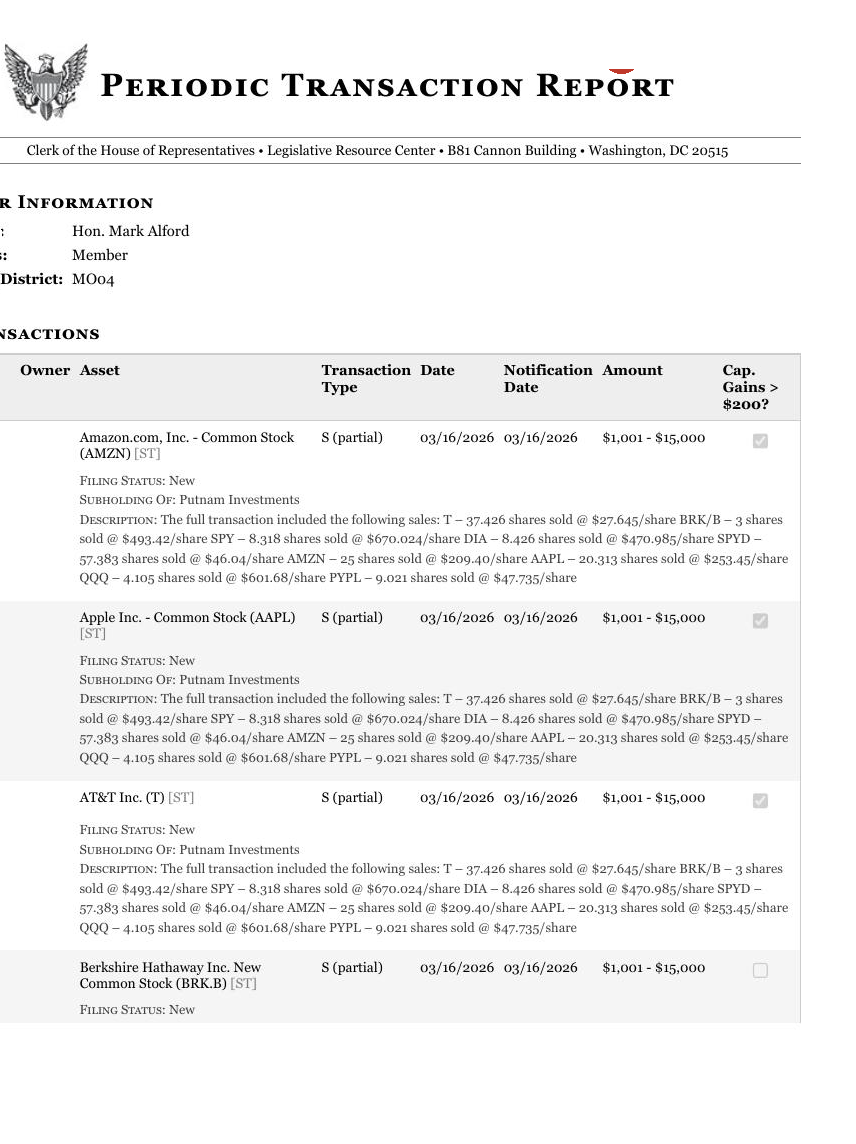
\includegraphics[height=7cm]{sources/house_digital.png}\\[3pt]
{\footnotesize\textbf{(a) Chambre — électronique.} PTR (\emph{House Clerk})~: tableau texte, ticker entre
parenthèses (AMZN), type d'actif entre crochets.}
\end{minipage}\hfill
\begin{minipage}[t]{0.47\textwidth}\centering
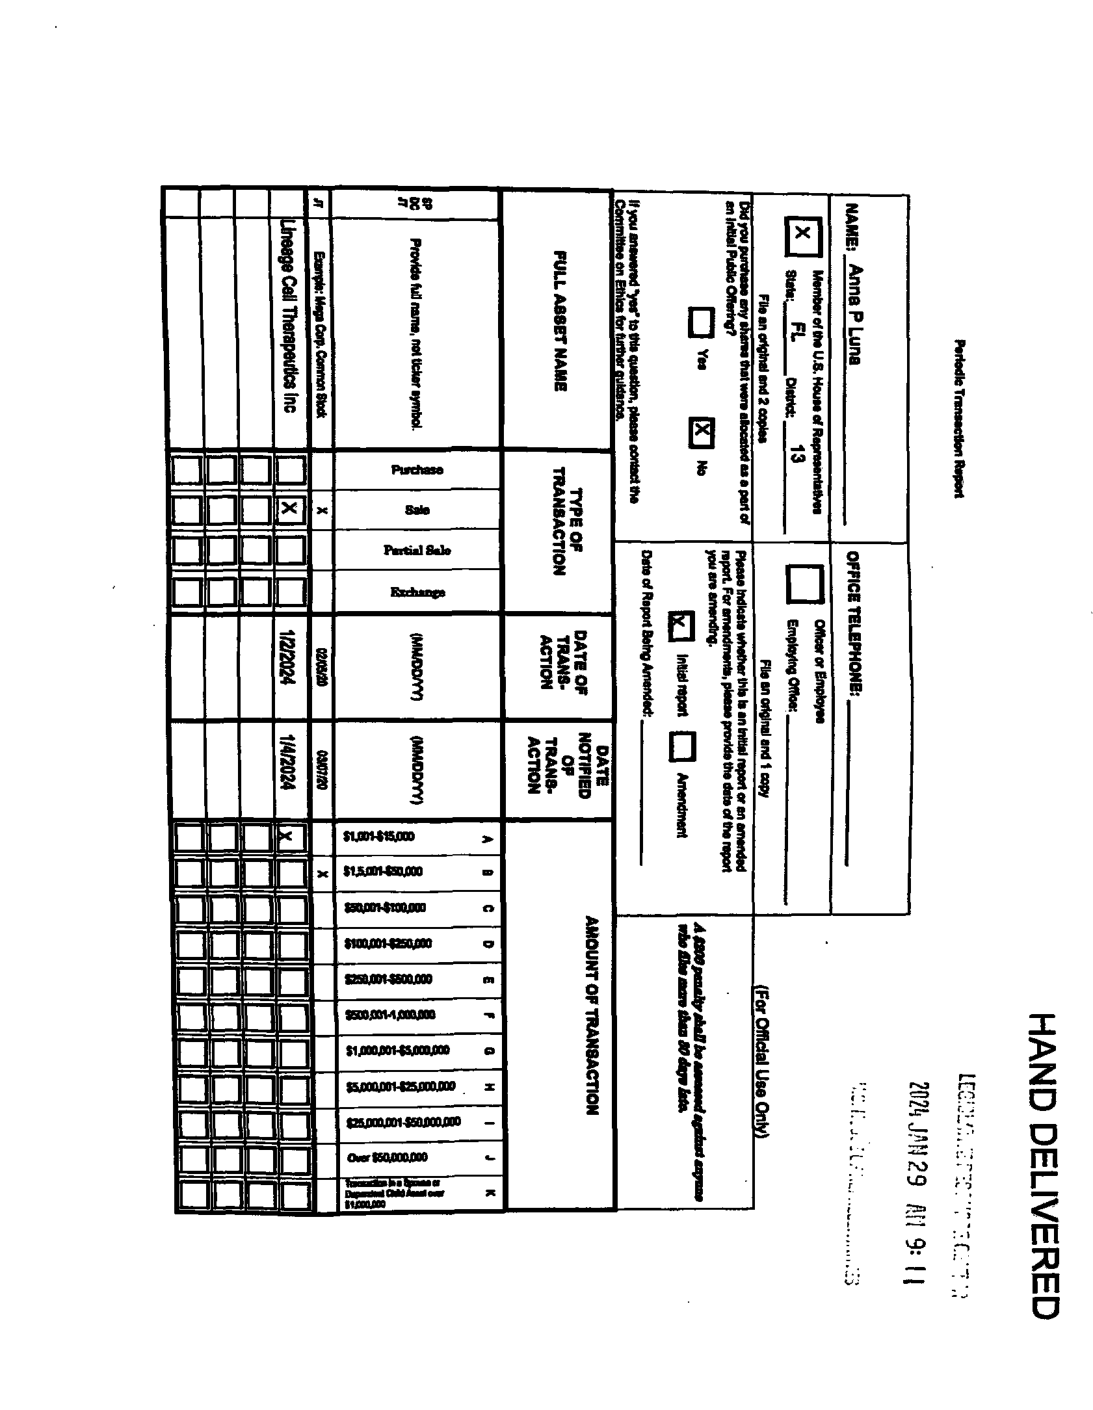
\includegraphics[height=7cm]{sources/house_ocr.png}\\[3pt]
{\footnotesize\textbf{(b) Chambre — OCR.} PDF scanné, ici \emph{couché}~: formulaire à cases, redressé
par deskew avant lecture Vision.}
\end{minipage}

\vspace{12pt}
\begin{minipage}[t]{0.47\textwidth}\centering
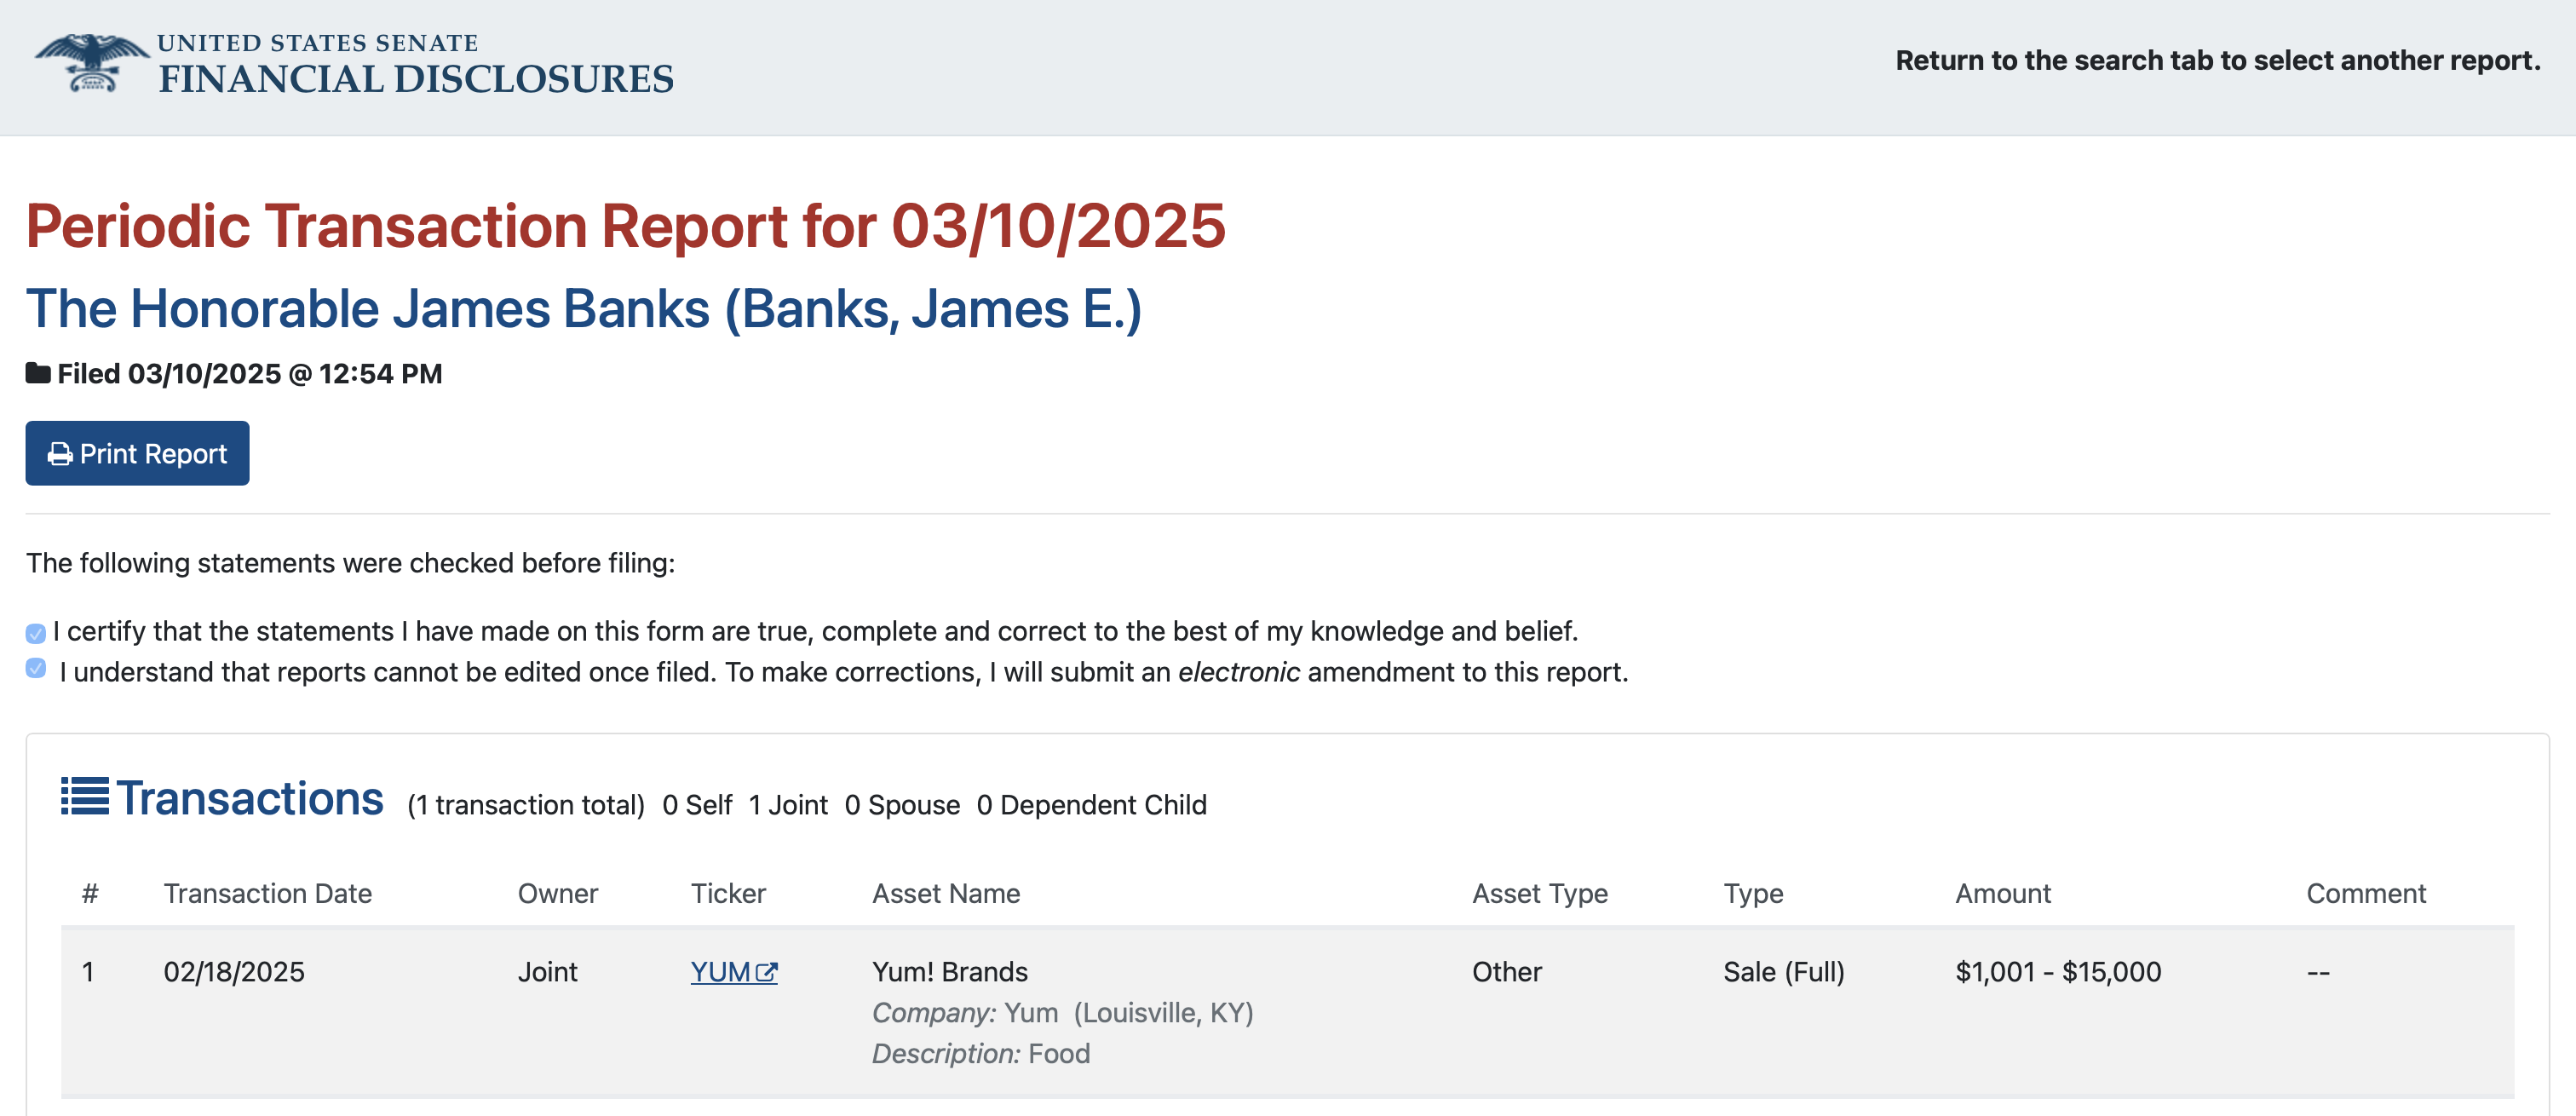
\includegraphics[width=\linewidth]{sources/senate_digital.png}\\[3pt]
{\footnotesize\textbf{(c) Sénat — électronique.} Page web eFD~: ticker cliquable (YUM), type d'opération
et montant — lue par \co{pd.read_html}.}
\end{minipage}\hfill
\begin{minipage}[t]{0.47\textwidth}\centering
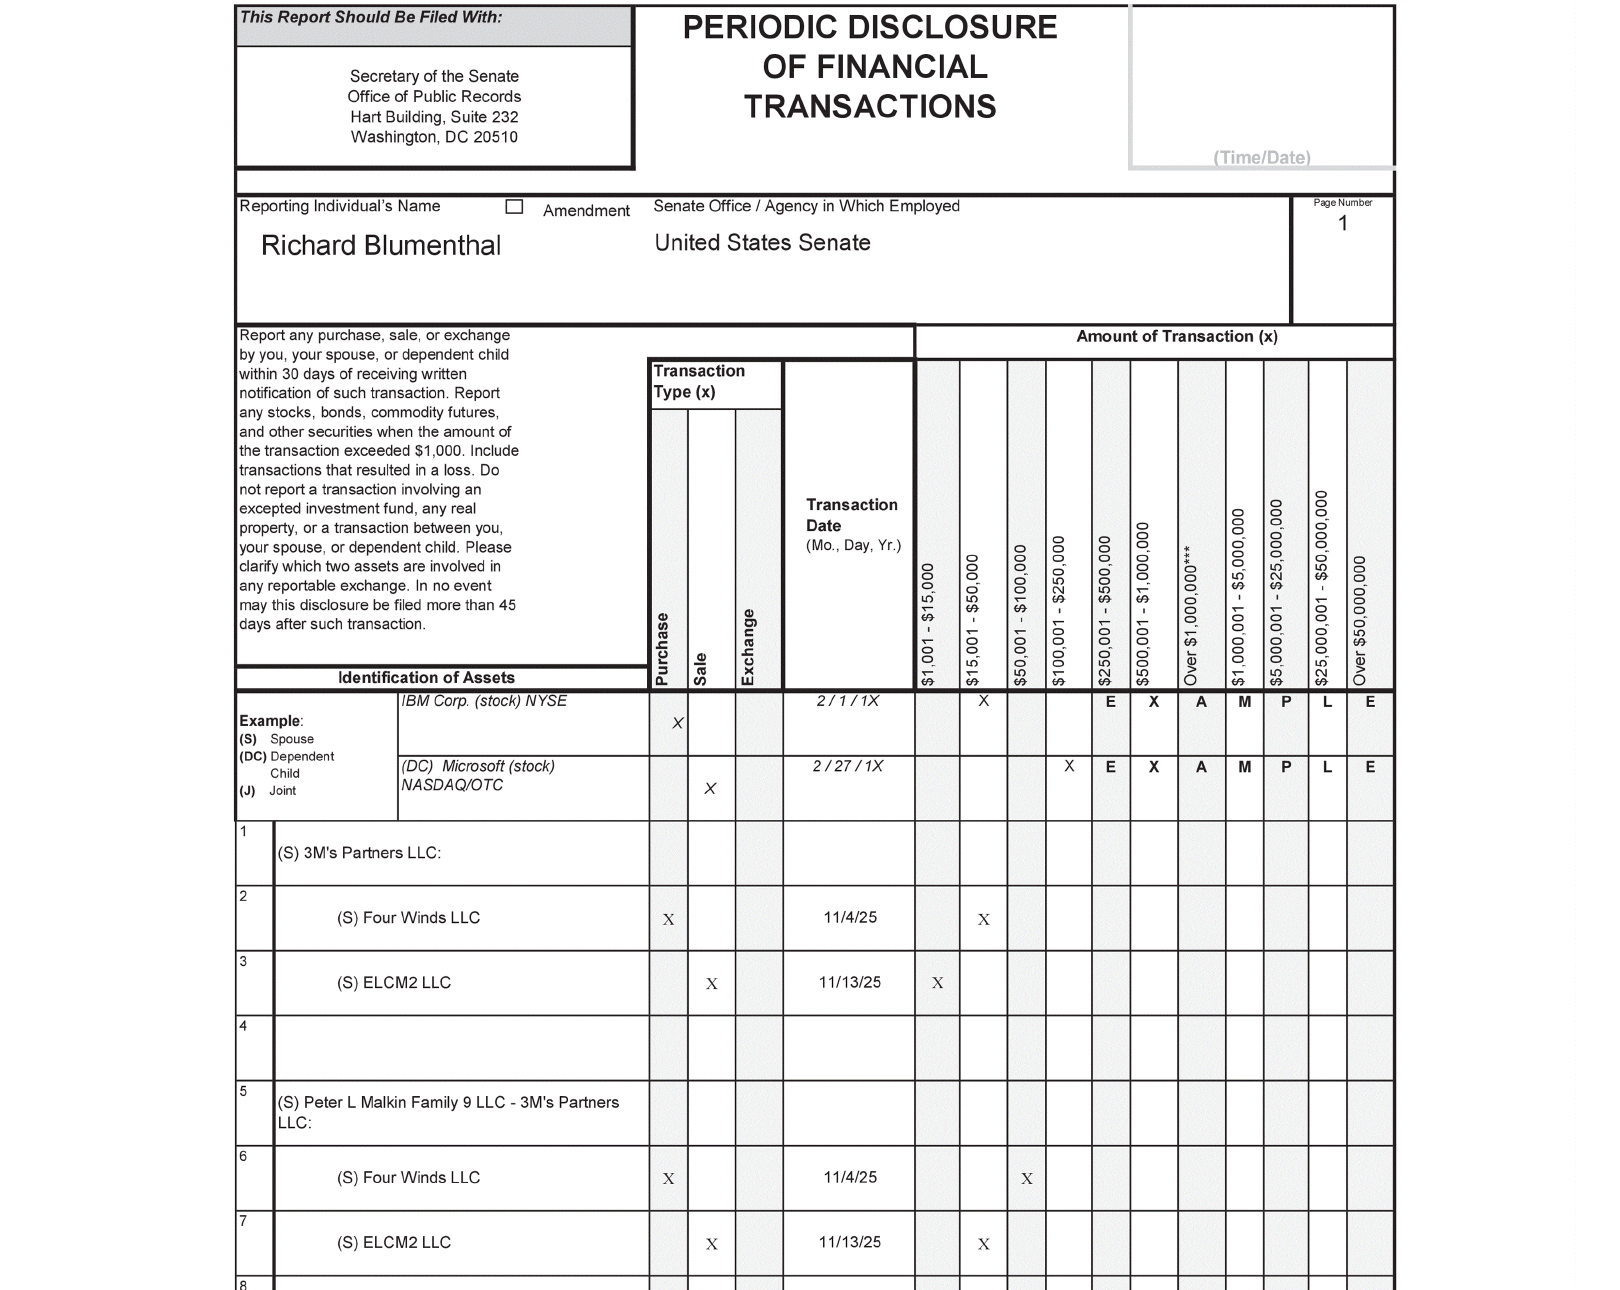
\includegraphics[width=\linewidth]{sources/senate_ocr.png}\\[3pt]
{\footnotesize\textbf{(d) Sénat — OCR.} Formulaire papier scanné (eFD \emph{media})~: lignes à cocher,
fourchettes de montant en colonnes.}
\end{minipage}
\end{center}

\subsection{Annexe B — modules \& fonctions clés}
\label{anx:modules}
Pour chaque module~: son rôle, et ses \textbf{fonctions centrales} (les helpers privés mineurs sont
omis). Le code vit dans \textbf{24 modules} (\co{common/} 9 + \co{house/} 7 + \co{senate/} 8)~;
l'orchestration se lit dans \co{common/pipeline.py:build_steps}, puis \co{house/digital.py:run_year},
\co{house/ocr.py:run_ocr_year}, \co{senate/digital.py:run_year} et \co{senate/fusion.py:main}.
{\footnotesize
\begin{longtable}{>{\ttfamily\footnotesize}p{2.4cm} p{4.0cm} p{8.8cm}}
\toprule
\normalfont\bfseries Module & \bfseries Rôle & \normalfont\bfseries Fonctions clés \\
\midrule\endhead
\multicolumn{3}{l}{\bfseries\color{coreC} common/ — le contrat universel partagé (9)}\\
reference.py & référentiel des élus & \co{load_reference} · \co{Reference} · \co{enrich_identity} · \co{add_years_in_office} · \co{bio_to_committees} \\
schema.py & clé naturelle + dédup & \co{natural_key_hash} (SHA-256 de 7 champs) · \co{add_occurrence_index} · \co{dedup_canonical} (non destructrice) · \co{CORE_FIELDS} \\
sector_enrich.py & secteur GICS → ETF & \co{resolve_yfinance} · \co{resolve_llm} (\co{is_listed}) · \co{enrich_sectors} (+ \co{sector_source}) · \co{GICS_TO_ETF} \\
vision_ocr.py & OCR Vision de référence & \co{detect_rotation} (deskew 4 rotations) · \co{pdf_to_b64_images} · \co{VisionExtractor.prompt_sha} · \co{.extract_cached} \\
crosscheck.py & statut par déposant & \co{per_filer_status} · \co{add_external_counts} (Kadoa/HSW) · \co{summary} \\
quality.py & rapport qualité (6 contrôles) & \co{load_final} · \co{date_coherence} · \co{delay_buckets} · \co{amount_distribution} · \co{coverage_per_member} · \co{unmatched_purchase_rate} · \co{quiver_validation} · \co{build_report} \\
enrich_tenure.py & ancienneté & \co{add_years_in_office} (append \co{years_in_office} octet-préservant) · \co{main} \\
pipeline.py & orchestrateur & \co{build_steps} (séquence 6 étapes) · \co{main} (sous-processus, \co{--dry-run}) \\
quiver_scopes.py & validation Quiver multi-scopes & \co{reconcile_scopes} (digital/ocr/both → \co{07c--07f}) · \co{match_breakdown} (par actif \& cluster → \co{07g}/\co{07h}) \\
\midrule
\multicolumn{3}{l}{\bfseries\color{houseC} house/ — orchestrateur Chambre (7)}\\
digital.py & PTR électroniques & \co{load_ptr_index} (XML, \co{FilingType=P}) · \co{resolve_pdf_path} · \co{build_manifest} (tri lisible/non) · \co{parse_ptr} (\co{TXN_RE}, \co{_join_split_lines}) · \co{finalize} · \co{validate_quiver} · \co{run_year} \\
ocr.py & scans → FINAL (par an) & \co{run_ocr_year} (Vision + fusion + ticker + secteur + Quiver 07c--07h) · \co{_infer_asset_type} \\
identity.py & matcher Chambre & \co{make_matcher} (override→exact+surnoms→nom unique) · \co{_MANUAL_BIO} \\
amounts.py & montant \& opération & \co{amount_midpoint} (milieu de fourchette) · \co{operation_type_from_code} (P/S/E) · \co{HOUSE_OCR_AMOUNT_MAP} \\
tickers.py & ticker + type d'actif & \co{explicit_ticker} · \co{recover_ticker} · \co{infer_asset_type} (par chambre) \\
quiver.py & réconciliation Quiver & \co{reconcile} · \co{norm_ticker} (robuste NaN/vide) \\
echantillon.py & pilote OCR stratifié & \co{run_echantillon} · \co{compare_quiver} \\
\midrule
\multicolumn{3}{l}{\bfseries\color{senateC} senate/ — orchestrateur Sénat (8)}\\
digital.py & eFD électronique & \co{accept_agreement} (CSRF) · \co{fetch_ptr_list} (\co{report_types=[11]}) · \co{fetch_report} · \co{parse_electronic} (\co{pd.read_html}, \co{_find_col}) · \co{run_year} \\
ocr.py & papier \co{.gif} → 06b & \co{discover_index} · \co{ocr_one} (un \co{.gif} → Vision) · \co{build_table} \\
ocr_engine.py & moteur OCR figé & \co{extract_report} · \co{normalize} · \co{_infer_asset_type} \\
fusion.py & fusion + enrich corpus & \co{main} (Étape 1 fusion/an · Étape 2 enrichissement corpus + Quiver 07c--07g) · \co{date_confidence} \\
identity.py & matcher Sénat & \co{load_reference} · \co{make_matcher} (désambiguïsation chambre, exclut délégués) · \co{enrich} \\
ticker.py & ticker 3 voies & \co{resolve_tickers} (explicit→dict→LLM) · \co{llm_resolve_tickers} \\
quiver.py & réconciliation Quiver & \co{reconcile} · \co{norm_ticker} · \co{norm_sense} \\
census_probe.py & Phase 0 (census) & \co{parse_electronic} · \co{main} (census + sondage parser) \\
\bottomrule
\end{longtable}}
\textit{Les \co{__init__.py} (exports de paquet) et \co{tests/regression/} (golden + reproductions)
complètent le dépôt. Le secteur (\co{common/sector_enrich}) et la clé (\co{common/schema}) sont importés
\emph{en direct} par les deux orchestrateurs — d'où leur place dans \co{common/}.}

\subsection{Annexe C — le schéma FINAL (28 colonnes)}
\label{anx:schema}
{\footnotesize
\begin{longtable}{r >{\ttfamily}p{3.3cm} p{8.2cm} >{\ttfamily\scriptsize}p{3.0cm}}
\toprule
\# & \normalfont\bfseries Colonne & \bfseries Sens & \normalfont\bfseries Remplie par \\
\midrule\endhead
1 & bioguide_id & identifiant officiel du membre & identity \\
2 & declarant_name & nom tel que déposé & parse / OCR \\
3 & chamber & \co{house} / \co{senate} & enrich_identity \\
4 & party & parti & Reference.party \\
5 & state_district & état + district & 03\_ptr\_index \\
6 & committee_membership & commissions (liste) & Reference.committees \\
7 & committees_key_flag & commission « clé » ? & reference \\
8 & transaction_date & date de la transaction & parse / OCR \\
9 & disclosure_date & date de divulgation (dépôt) & 03\_ptr\_index / eFD \\
10 & ticker & symbole boursier & tickers / ticker \\
11 & asset_description & libellé de l'actif & parse / OCR \\
12 & asset_type & type d'actif & infer_asset_type \\
13 & sector_gics & secteur GICS & sector_enrich \\
14 & etf_proxy & ETF SPDR du secteur & GICS\_TO\_ETF \\
15 & operation_type & Purchase / Sale / … & operation_type_from_code \\
16 & amount_range & fourchette déclarée & parse / OCR \\
17 & amount_midpoint & milieu de la fourchette & amount_midpoint \\
18 & amount_split_flag & lot multi-actifs ? & finalize \\
19 & owner & propriétaire (self/spouse…) & normalize \\
20 & doc_id & identifiant du PTR & 03\_ptr\_index \\
21 & source_url & URL de la source & 03\_ptr\_index \\
22 & natural_key_hash & clé de dédup (7 champs) & schema \\
23 & occurrence_index & rang du lot intra-dépôt & add_occurrence_index \\
24 & provenance & \co{*-electronic} / \co{*-ocr} & pipeline \\
25 & date_confidence & plausible / implausible (75 j) & date_confidence \\
26 & ticker_source & explicit / elec\_dict / llm / none & tickers / ticker \\
27 & sector_source & yfinance / llm / manual / none & sector_enrich \\
28 & years_in_office & ancienneté à la date du trade & enrich_tenure \\
\bottomrule
\end{longtable}}
\textit{L'ordre exact diffère légèrement entre Chambre et Sénat (\co{date_confidence} plus tôt au
Sénat)~; le contenu garanti — les 12 champs « métier » — est identique. Les 27 colonnes d'assemblage
(\co{HOUSE_FINAL_SCHEMA} / \co{SENATE_FINAL_SCHEMA}) + \co{years_in_office} = 28.}

\subsection{Annexe D — métriques vérifiées (recalculées depuis les FINAL)}
\label{anx:metrics}
\textbf{Lue après le rapport, cette annexe dit si l'extraction a bien marché.} Tous les chiffres sont
recomputés depuis les tables FINAL par \co{tests/regression/audit_metrics.py}, \co{common/quality.py} et
les réconciliations Quiver figées (\co{07c--07h}).

\textbf{D.1 — Volumes par an.}
\begin{center}\small
\begin{tabular}{l rrrr @{\hspace{1.4em}} rrrr}
\toprule
& \multicolumn{4}{c}{\bfseries\color{houseC}Chambre} & \multicolumn{4}{c}{\bfseries\color{senateC}Sénat}\\
\cmidrule(lr){2-5}\cmidrule(lr){6-9}
\bfseries An & élec. & OCR & FINAL & dépos. & élec. & OCR & FINAL & sén.\\
\midrule
2020 & 6\,886 & 8\,791 & 15\,677 & 109 & 1\,706 & 255 & 1\,961 & 33 \\
2021 & 5\,457 & 6\,816 & 12\,273 & 120 & 1\,098 & 281 & 1\,379 & 35 \\
2022 & 3\,601 & 10\,900 & 14\,501 & 110 & 919 & 182 & 1\,101 & 27 \\
2023 & 4\,161 & 6\,329 & 10\,490 & 100 & 1\,062 & 97 & 1\,159 & 30 \\
2024 & 2\,694 & 6\,277 & 8\,971 & 97 & 946 & 84 & 1\,030 & 24 \\
2025 & 7\,577 & 6\,067 & 13\,644 & 107 & 943 & 478 & 1\,421 & 31 \\
2026 & 2\,300 & 3\,790 & 6\,090 & 84 & 487 & 303 & 790 & 22 \\
\midrule
\bfseries Tot. & \bfseries 32\,676 & \bfseries 48\,970 & \bfseries 81\,646 & \bfseries 256$^\ast$ & \bfseries 7\,161 & \bfseries 1\,680 & \bfseries 8\,841 & \bfseries 64$^\ast$\\
\bottomrule
\end{tabular}
\end{center}
{\footnotesize $^\ast$ bioguides \emph{uniques} sur 7 ans (la somme annuelle compte un élu chaque année).}

\textbf{D.2 — Couverture des champs enrichis, par an (\% renseigné).}
\begin{center}\small
\begin{tabular}{l rrrr @{\hspace{1.2em}} rrrr}
\toprule
& \multicolumn{4}{c}{\bfseries\color{houseC}Chambre} & \multicolumn{4}{c}{\bfseries\color{senateC}Sénat}\\
\cmidrule(lr){2-5}\cmidrule(lr){6-9}
\bfseries An & ticker & sect. & a.type & comm. & ticker & sect. & a.type & comm.\\
\midrule
2020 & 86,5 & 83,4 & 91,0 & 64,9 & 88,1 & 80,5 & 96,3 & 34,5 \\
2021 & 87,3 & 85,8 & 90,1 & 78,7 & 80,9 & 70,1 & 94,2 & 54,3 \\
2022 & 87,1 & 85,2 & 91,0 & 89,2 & 79,7 & 65,3 & 96,1 & 78,3 \\
2023 & 78,9 & 76,6 & 88,6 & 96,8 & 77,7 & 69,5 & 96,3 & 71,4 \\
2024 & 81,3 & 78,3 & 87,4 & 93,6 & 68,0 & 59,2 & 100 & 77,8 \\
2025 & 87,8 & 86,3 & 94,8 & 97,6 & \textbf{45,4} & \textbf{37,2} & 100 & 84,9 \\
2026 & 85,4 & 84,4 & 94,9 & 99,7 & \textbf{43,7} & \textbf{35,7} & 100 & 86,2 \\
\midrule
\bfseries Glob. & \bfseries 85,3 & \bfseries 83,2 & \bfseries 91,1 & \bfseries 86,6 & \bfseries 71,4 & \bfseries 62,1 & \bfseries 97,3 & \bfseries 65,6 \\
\bottomrule
\end{tabular}
\end{center}

\textbf{D.3 — Les 6 contrôles qualité} (global).
\begin{center}\small
\begin{tabular}{p{8.4cm} r r}
\toprule
\bfseries Contrôle & \bfseries Chambre & \bfseries Sénat\\
\midrule
(a) dates cohérentes (\co{disclosure ≥ transaction}) & 99,8\,\% & 100,0\,\% \\
(b) dépôts ≤ 45 j (délai médian 28 j) & 86,9\,\% & 84,9\,\% \\
(c) montants — médiane / quartile haut & \multicolumn{2}{c}{8\,000\,\$ / 32\,500\,\$} \\
(d) déposants (≥ 10 trades / ≥ 3 ans) & \multicolumn{2}{c}{320 (206 / 150)} \\
(e) achats sans sortie déclarée & 22,5\,\% & 39,6\,\% \\
(f) validation Quiver — scope « les deux » & 86,2\,\% & 99,4\,\% \\
\bottomrule
\end{tabular}
\end{center}

\textbf{D.4 — Validation Quiver par scope, par an} (couverture \% = trades Quiver retrouvés ;
\co{common/quiver_scopes.py}).
\begin{center}\small
\begin{tabular}{l rrr @{\hspace{1.6em}} rrr}
\toprule
& \multicolumn{3}{c}{\bfseries\color{houseC}Chambre} & \multicolumn{3}{c}{\bfseries\color{senateC}Sénat}\\
\cmidrule(lr){2-4}\cmidrule(lr){5-7}
\bfseries An & élec. & OCR & les deux & élec. & OCR & les deux\\
\midrule
2020 & 99,7 & 61,3 & 85,1 & 99,4 & — & 99,4 \\
2021 & 99,6 & 56,0 & 88,6 & 98,0 & — & 98,0 \\
2022 & 98,2 & 68,5 & 80,9 & 99,4 & — & 99,4 \\
2023 & 96,0 & 67,1 & 81,0 & 99,7 & 0,0 & 99,7 \\
2024 & 92,0 & 78,8 & 85,8 & 99,6 & 0,0 & 99,6 \\
2025 & 99,2 & 61,2 & 91,3 & 99,8 & — & 99,8 \\
2026 & 98,6 & 85,3 & 90,6 & 100,0 & — & 100,0 \\
\midrule
\bfseries Glob. & \bfseries 98,2 & \bfseries 68,3 & \bfseries 86,2 & \bfseries 99,4 & \bfseries 0,0 & \bfseries 99,4 \\
\bottomrule
\end{tabular}
\end{center}
{\footnotesize Le scope OCR du Sénat est « — » (Quiver ne possède aucun de ces trades~: ce sont surtout
des munis non cotées). Le scope « les deux » est l'\emph{union dédupliquée}, pas la somme.}

\textbf{D.5 — Décomposition Quiver par type d'actif et par cluster} (toutes années~; \co{07g}/\co{07h}).
\begin{center}\small
\begin{tabular}{l rrrr r}
\toprule
\bfseries Chambre — type d'actif & exact & date\,$\neq$ & no\_match & non\_equity & Quiver a\,\%\\
\midrule
Stock & 47\,475 & 9\,301 & 8\,105 & 2\,796 & \textbf{87,5} \\
Mutual Fund & 130 & 92 & 715 & 575 & 23,7 \\
Gov Security & 5 & 0 & 23 & 2\,259 & 17,9 \\
\midrule
\bfseries Cluster de scan & exact & date\,$\neq$ & no\_match & non\_equity & date juste\,\%\\
\midrule
A — tapé droit & 3\,784 & 630 & 600 & 943 & \textbf{85,7} \\
B — tapé couché & 18\,558 & 8\,653 & 7\,706 & 7\,234 & \textbf{68,2} \\
C — manuscrit & 100 & 169 & 493 & 100 & \textbf{37,2} \\
\bottomrule
\end{tabular}
\end{center}
{\footnotesize \emph{Quiver a\,\%} = (exact + date\,$\neq$) / actions~; \emph{date juste\,\%} = exact /
(exact + date\,$\neq$). Sénat~: les \co{Stock} sont couverts à 84,2\,\%~; l'OCR y est surtout du non-coté
(Municipal Security, Corporate Bond) → hors périmètre Quiver.}

\textbf{D.6 — Fiabilité des dates OCR (\co{date_confidence}, lignes OCR seulement).}
\begin{center}\small
\begin{tabular}{l rr @{\hspace{1.6em}} rr}
\toprule
& \multicolumn{2}{c}{\bfseries\color{houseC}Chambre (OCR)} & \multicolumn{2}{c}{\bfseries\color{senateC}Sénat (OCR)}\\
\cmidrule(lr){2-3}\cmidrule(lr){4-5}
\bfseries An & plausible\,\% & implausibles & plausible\,\% & implausibles\\
\midrule
2020 & 98,6 & 120 & 96,1 & 9 \\
2021 & \textbf{79,6} & \textbf{1\,389} & 97,5 & 6 \\
2022 & 96,4 & 394 & 99,5 & 0 \\
2023 & 99,2 & 50 & 100,0 & 0 \\
2024 & 96,5 & 220 & 97,6 & 0 \\
2025 & 98,1 & 118 & 99,0 & 3 \\
2026 & 100,0 & 0 & 99,7 & 0 \\
\midrule
\bfseries Tot. & \bfseries 95,3 & \bfseries 2\,291 & \bfseries 98,5 & \bfseries 18 \\
\bottomrule
\end{tabular}
\end{center}
{\footnotesize Le creux 2021 Chambre est entièrement Diana Harshbarger (2 documents manuscrits denses).}

\textbf{D.7 — Clusters OCR \& concentration.}
\begin{center}\small
\begin{tabular}{p{7.2cm} p{8.2cm}}
\toprule
\bfseries Clusters Chambre (census 547 scans) & \bfseries Concentration des déposants OCR\\
\midrule
A — tapé droit : 74 docs & Chambre : Khanna 30\,862 (62,9\,\%), McCaul 10\,876 (22,2\,\%),\\
B — tapé couché : 322 docs & \quad Harshbarger 3\,514 (7,2\,\%) → top~3 = 92,4\,\%, top~10 = 99,0\,\%\\
C — manuscrit : 151 docs (exclu) & Sénat : Blumenthal 1\,233 (73\,\%), Boozman 379, Burr 52,\\
 & \quad Feinstein 14, Fetterman 2\\
\bottomrule
\end{tabular}
\end{center}

\textbf{D.8 — Statut de validation par déposant (Chambre, \co{crosscheck}).}
\begin{center}\small
\begin{tabular}{l rrr}
\toprule
\bfseries Statut & \bfseries déposants & \bfseries transactions & \bfseries dont OCR\\
\midrule
\co{quiver_validable} (Quiver le couvre) & 212 & 78\,530 & 47\,004 \\
\co{ocr_unique} (Quiver = 0, OCR $\geq$ 50\,\%) & 13 & 1\,957 & 1\,949 \\
\co{digital} (peu / pas d'OCR) & 31 & 1\,155 & 13 \\
\bottomrule
\end{tabular}
\end{center}
{\footnotesize Identité~: Chambre 256 bioguides / 275 noms (99,99\,\%), Sénat 64 / 67 (100\,\%). Golden
(zéro écart)~: \textbf{125} fichiers Chambre, \textbf{76} Sénat. \textbf{Total~: 90\,487 transactions},
2020--2026.}

\subsection{Annexe E — reproduire / lancer}
\label{anx:run}
{\footnotesize
\begin{verbatim}
# Installation
python3.12 -m venv .venv && ./.venv/bin/pip install -e .

# Pipeline complet (reseau + API Vision requis) ; --dry-run = voir la sequence
./.venv/bin/python -m common.pipeline --years 2020-2026
./.venv/bin/python -m common.pipeline --years 2024 --dry-run

# Rapport de qualite (offline, lecture seule des FINAL)
#   -> docs/RAPPORT_QUALITE.md + docs/quality/*.png
./.venv/bin/python -m common.quality

# Filet "zero changement" (doit afficher ZERO ECART)
./.venv/bin/python tests/regression/check_golden.py         # Chambre, 125
./.venv/bin/python tests/regression/senate_check_golden.py  # Senat,    76
./.venv/bin/python tests/regression/test_senate_repro.py    # reproductions
\end{verbatim}}

\vfill
\begin{center}\footnotesize\itshape
Document dérivé et vérifié sur le code source réel et les tables FINAL du dépôt. Toute divergence avec
une autre documentation doit être tranchée en faveur du code et des données. Quiver = vérification
externe, jamais réinjecté.
\end{center}

\end{document}
